\documentclass[a4paper,titlepage,11pt,floatssmall]{mwrep}
\usepackage[left=2.5cm,right=2.5cm,top=2.5cm,bottom=2.5cm]{geometry}
\usepackage[OT1]{fontenc}
\usepackage{polski}
\usepackage{amsmath}
\usepackage{amsfonts}
\usepackage{amssymb}
\usepackage{graphicx}
\usepackage{float}
\usepackage{subfig}
\usepackage{url}
\usepackage{tikz}
\usetikzlibrary{arrows,calc,decorations.markings,math,arrows.meta}
\usepackage{rotating}
\usepackage[percent]{overpic}
\usepackage[utf8]{inputenc}
\usepackage{xcolor}
\usepackage{colortbl}
\usepackage{listings}
\usepackage{matlab-prettifier}
\usepackage{enumitem,amssymb}
\definecolor{szary}{rgb}{0.95,0.95,0.95}
\usepackage{siunitx}
\sisetup{detect-weight,exponent-product=\cdot,output-decimal-marker={,},per-mode=symbol,range-phrase={-},range-units=single}

%konfiguracje pakietu listings
\lstset{
  literate={ą}{{\k a}}1
           {Ą}{{\k A}}1
           {ż}{{\. z}}1
           {Ż}{{\. Z}}1
           {ź}{{\' z}}1
           {Ź}{{\' Z}}1
           {ć}{{\' c}}1
           {Ć}{{\' C}}1
           {ę}{{\k e}}1
           {Ę}{{\k E}}1
           {ó}{{\' o}}1
           {Ó}{{\' O}}1
           {ń}{{\' n}}1
           {Ń}{{\' N}}1
           {ś}{{\' s}}1
           {Ś}{{\' S}}1
           {ł}{{\l}}1
           {Ł}{{\L}}1
}
\lstset{
	backgroundcolor=\color{szary},
	frame=single,
	breaklines=true,
}
\lstdefinestyle{customlatex}{
	basicstyle=\footnotesize\ttfamily,
	%basicstyle=\small\ttfamily,
}
\lstdefinestyle{customc}{
	breaklines=true,
	frame=tb,
	language=C,
	xleftmargin=0pt,
	showstringspaces=false,
	basicstyle=\small\ttfamily,
	keywordstyle=\bfseries\color{green!40!black},
	commentstyle=\itshape\color{purple!40!black},
	identifierstyle=\color{blue},
	stringstyle=\color{orange},
}
\lstdefinestyle{custommatlab}{
	captionpos=t,
	breaklines=true,
	frame=tb,
	xleftmargin=0pt,
	language=matlab,
	showstringspaces=false,
	basicstyle=\small\ttfamily,
	%basicstyle=\scriptsize\ttfamily,
	keywordstyle=\bfseries\color{green!40!black},
	commentstyle=\itshape\color{purple!40!black},
	identifierstyle=\color{blue},
	stringstyle=\color{orange},
}
\lstdefinestyle{custompython}{
	captionpos=t,
	breaklines=true,
	frame=tb,
	xleftmargin=0pt,
	language=python,
	showstringspaces=false,
	basicstyle=\small\ttfamily,	
	keywordstyle=\bfseries\color{green!40!black},
	commentstyle=\itshape\color{purple!40!black},
	identifierstyle=\color{blue},
	stringstyle=\color{orange},
}

%wymiar tekstu (bez żywej paginy)
\textwidth 160mm \textheight 247mm

\def\figurename{Rys.}
\def\tablename{Tab.}

%konfiguracja liczby pływających elementów
\setcounter{topnumber}{0}%2
\setcounter{bottomnumber}{3}%1
\setcounter{totalnumber}{5}%3
\renewcommand{\textfraction}{0.01}%0.2
\renewcommand{\topfraction}{0.95}%0.7
\renewcommand{\bottomfraction}{0.95}%0.3
\renewcommand{\floatpagefraction}{0.35}%0.5

\begin{document}
\frenchspacing
\pagestyle{uheadings}

%strona tytułowa
\title{\bf Zastosowanie modeli statyki typu Takagi-Sugeno z następnikami hiperbolicznymi w algorytmach regulacji predykcyjnej}
\author{Wojciech Rogalski}
\date{2024}

\makeatletter
\renewcommand{\maketitle}{\begin{titlepage}
\begin{center}{\LARGE {\bf
Wydział Elektroniki i Technik Informacyjnych}}\\
\vspace{0.4cm}
{\LARGE {\bf Politechnika Warszawska}}\\
\vspace{0.3cm}
\end{center}
\vspace{5cm}
\begin{center}
{\bf \LARGE Pracownia problemowa magisterska \vskip 0.1cm}
(semestr letni 23/24L)
\end{center}
\vspace{1cm}
\begin{center}
{\bf \LARGE \@title \vskip 0.1cm}
\end{center}
\vspace{2cm}
\begin{center}
\begin{tabular}{@{}c@{\hspace{2cm}}c@{}}
\bf \Large Autor: & \bf \Large Promotor: \\
\@author & dr hab. inż. Piotr Marusak
\end{tabular}
\end{center}
\vspace*{\stretch{6}}
\begin{center}
\bf{\large{Warszawa, \@date\vskip 0.1cm}}
\end{center}
\end{titlepage}
}
\makeatother
\maketitle
\tableofcontents

\chapter{Wstęp}
Praca zawiera porównanie modeli Hammersteina oraz Wienera w regulacji kaskadowej. Bazą porównania był obiekt opisany równaniami fizycznymi postaci:
\begin{equation}
\begin{cases}
\frac{dV_1}{dt} = F_1 + F_D - F_2(h_1) \\
\frac{dV_2}{dt} = F_2(h_1) - F_3(h_2) \\
F_2(h_1) = \alpha_1 \sqrt{h_1}, \quad F_3(h_2) = \alpha_2 \sqrt{h_2}, \quad V_1(h_1) = A_1h_1, \quad V_2(h_2) = C_2h_2^2, \quad F_1(t) = F_{1in}(t-\tau)  
\end{cases}
\label{model_fiz}
\end{equation}

\begin{itemize}
\item[•] Stałe: 
\begin{equation}
A_1 = 540cm^2, \quad C_2 = \num{0.85}, \quad \alpha_1 = 26, \quad \alpha_2 = 20
\end{equation}

\item[•] Punkt pracy:
\begin{equation}
F_1 = 90 \frac{cm^3}{s}, \quad F_D = 30 \frac{cm^3}{s}, \quad \tau = 100, \quad h_2 = 36cm
\end{equation}
\end{itemize}

\noindent gdzie użyte oznaczenia odpowiadają tym zastosowanym na rys. \ref{schemat}.

\begin{figure}[h!]
\centering
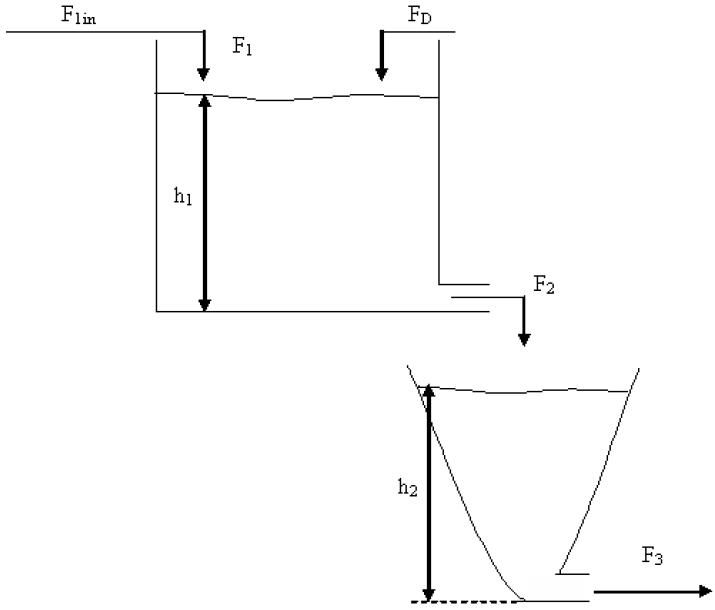
\includegraphics[width=0.8\textwidth]{pictures/schemat}
\caption{Obiekt regulacji automatycznej.}
\label{schemat}
\end{figure}

Wartością sterującą był dopływ $F_{1in}$ natomiast zakłóceniem - $F_D$. Z kolei wyjściem - wartością regulowaną - wysokość cieczy w drugim zbiorniku $h_2$. W pierwszej kolejności dokonano identyfikacji modelu, sprawdzono jego nieliniowość i dobrano odpowiedni rząd dynamiki modelu liniowego.
\chapter{Identyfikacja}
\section{Charakterystyka statyczna}
Poświęcono jej bardzo dużo uwagi, ze względu na kluczową rolę, jaką odgrywa we wspomnianych modelach Hammersteina i Wienera. Korzystając z modelu fizycznego, z równania \ref{model_fiz} wyznaczono:
\begin{equation}
\frac{dV_1}{dt} = 0 \quad \wedge \quad \frac{dV_2}{dt} = 0
\end{equation}

\noindent wobec tego:
\begin{equation}
\begin{cases}
F_1 + F_D - \alpha_1 \sqrt{h_1} &= 0 \\
\alpha_1 \sqrt{h_1} - \alpha_2 \sqrt{h_2} &= 0
\end{cases}
\end{equation}

\noindent Po prostych przekształceniach otrzymano wzór opisujący charakterystykę statyczną:
\begin{equation}
h_2 = \left( \frac{F_1 + F_D}{\alpha_2} \right)^2
\end{equation}

\noindent Wykres odpowiadający wyprowadzonemu wzorowi prezentuje się następująco:

\begin{figure}[h!]
\centering
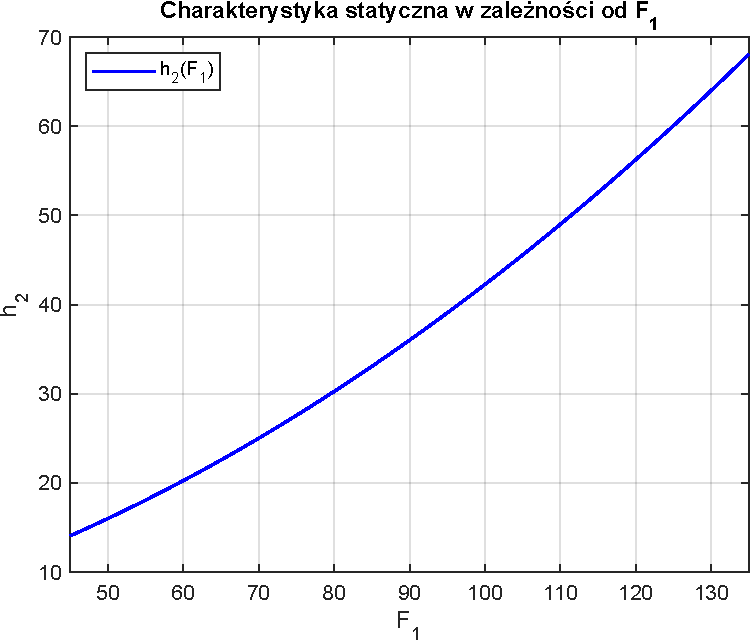
\includegraphics[width=0.8\textwidth]{pictures/static_characteristic}
\caption{Charakterystyka statyczna $h_2(F_1)$.}
\label{static_characteristic}
\end{figure}

\noindent Założono przedział zmienności sygnału sterującego w zakresie $F_1 \in [-45, 45]$.

\newpage

\section{Wymuszenia}
Po dokonaniu pierwszego kroku identyfikacji - wykreślenia charakterystyki statycznej - uzyskano wstępne informacje o obiekcie. Równania opisujące model (\ref{model_fiz}) oraz charakterystyka statyczna przedstawiona na rys. \ref{static_characteristic} pokazuje, że obiekt jest nieliniowy, stąd dokonano jego linearyzacji w punkcie pracy, tj.:
\begin{equation}
\begin{cases}
\frac{dV_1}{dt} \cong F_1 + F_D - \alpha_1 \sqrt{\frac{V_{10}}{A}} - \frac{\alpha_1}{2 \sqrt{A \cdot V_{10}}} \cdot (V_1 - V_{10})\\
\frac{dV_2}{dt} \cong \alpha_1 \sqrt{\frac{V_{10}}{A}} - \alpha_2 \sqrt[4]{\frac{V_{20}}{C}} + \frac{\alpha_1}{2 \sqrt{A \cdot V_{10}}} \cdot (V_1 - V_{10}) - \frac{\alpha_2}{4 \sqrt[4]{C \cdot V_{20}^3}} \cdot (V_2 - V_{20})
\end{cases}
\end{equation}

\noindent Linearyzacji dokonano przyjmując jako zmienną stanu objętość cieczy w obu zbiornikach. 

\begin{equation}
x = \begin{bmatrix} V_1 & V_2 \end{bmatrix}^T
\end{equation}

Następnie, podając wygenerowaną sekwencję sygnału sterującego, zbadano rozbieżność modelu liniowego i nieliniowego.

\begin{figure}[h!]
\centering
\subfloat[Wygenerowana sekwencja sygnału sterującego $u(k)$.]{
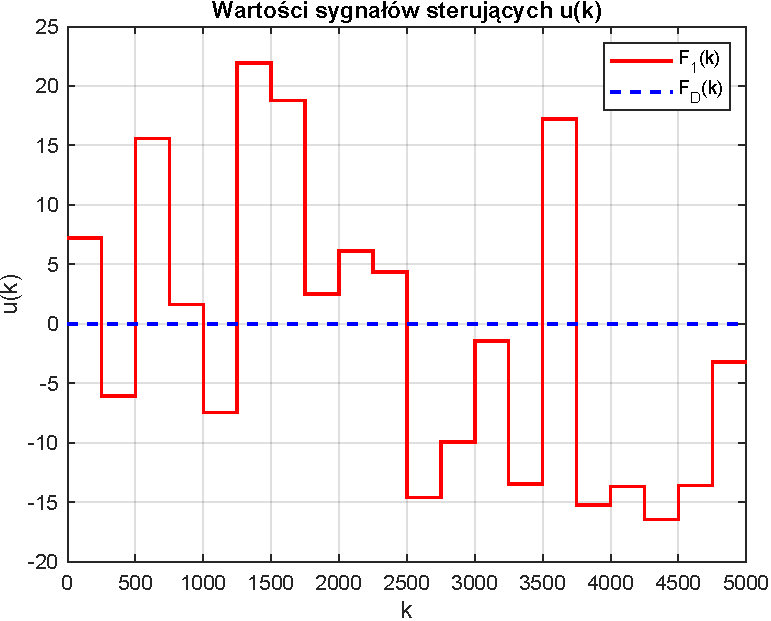
\includegraphics[width=0.45\textwidth]{pictures/u_F1}}
\hfill
\subfloat[Sygnał wyjściowy $y(k)$.]{
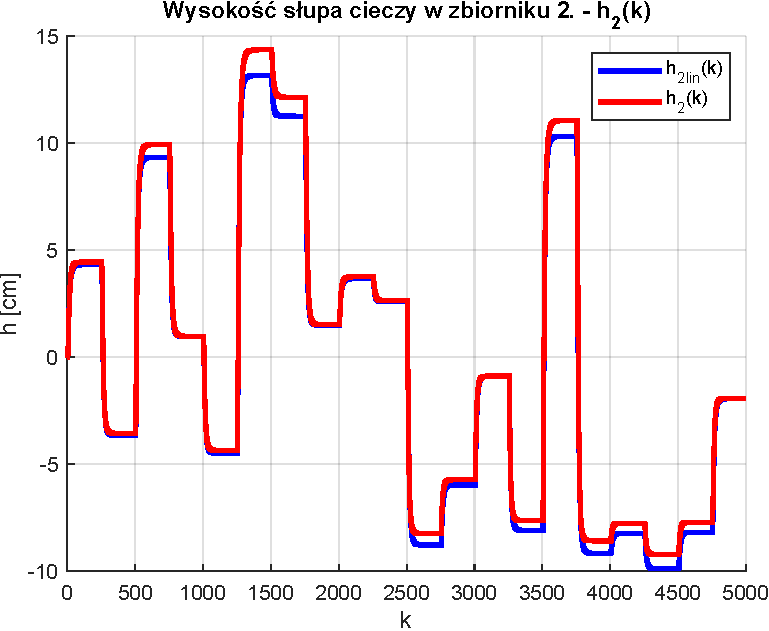
\includegraphics[width=0.45\textwidth]{pictures/y_F1}}
\caption{Porównanie modelu liniowego z nieliniowym.}
\end{figure}

Otrzymano dokładnie to czego się spodziewano. Wymuszenia nie większe niż $\pm 10 \frac{cm^3}{s}$ nie powodują znacznego wytrącenia układu z położenia równowagi, dzięki czemu model liniowy bardzo dobrze aproksymuje zachowanie układu. Niestety sytuacja pogarsza się wraz z oddalaniem się od punktu pracy - model liniowy zaczyna poważnie odbiegać od modelu nieliniowego, opisującego obiekt. W celach porównawczych policzono błędy, testując model w trybie bez rekurencji (ARX) oraz z rekurencją OE, przyjmując jako kryterium jakości błąd średni kwadratowy, tj.:

\begin{equation}
E = \sum_{k=0}^N (y(k) - y^{mod}(k))^2
\end{equation}

\noindent Wcześniej dokonano podziału wygenerowanych danych dynamicznych na dwa zbiory - uczący i~weryfikujący - stosując zasadę podziału $0\% - 50\% / 50\% - 100\%$, potrzebne do późniejszego, ewentualnego dostrajania modelu. Otrzymano następujące wyniki:

\begin{description}
\item[ARX] 
\begin{equation}
E_{ucz} = \num{0.002} \hspace{1cm} E_{wer}=\num{0.003}
\end{equation}
\item[OE] 
\begin{equation}
E_{ucz} = \num{0.470} \hspace{1cm} E_{wer}=\num{0.831}
\end{equation}
\end{description}

%\newpage

\begin{figure}[p!]
\begin{center}
\Large \textbf{Model ARX}
\end{center} 
\centering
\subfloat[Zbiór uczący.]{
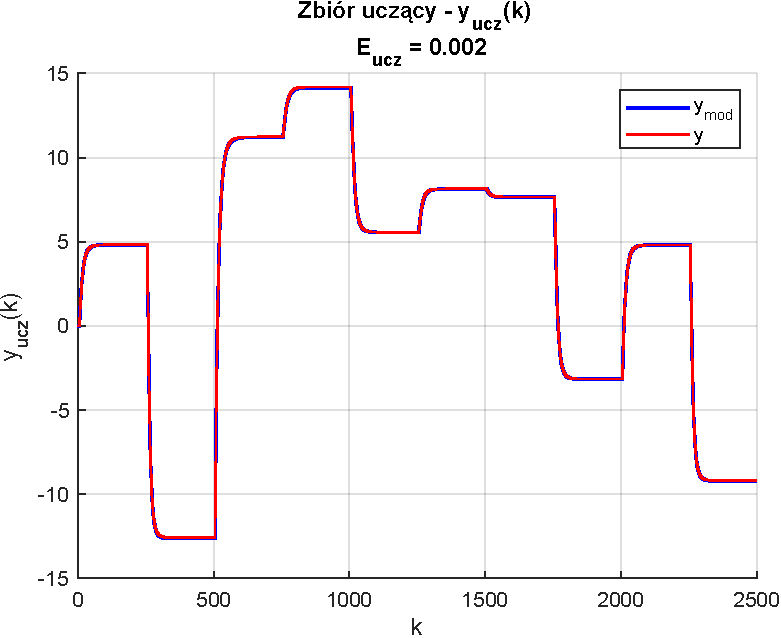
\includegraphics[width=0.45\textwidth]{pictures/arx_ucz}}
\hfill
\subfloat[Zbiór weryfikujący.]{
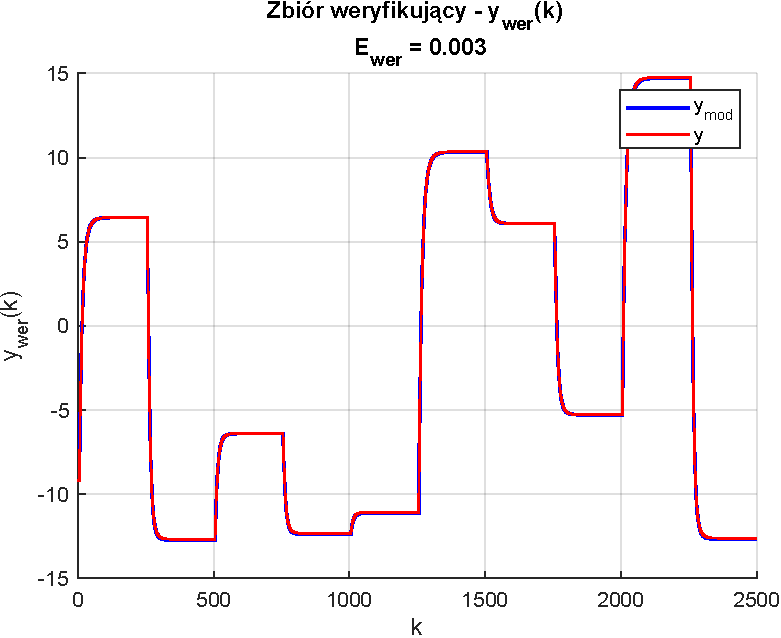
\includegraphics[width=0.45\textwidth]{pictures/arx_wer}}

\begin{center}
\Large \textbf{Model OE}
\end{center} 
\subfloat[Zbiór uczący.]{
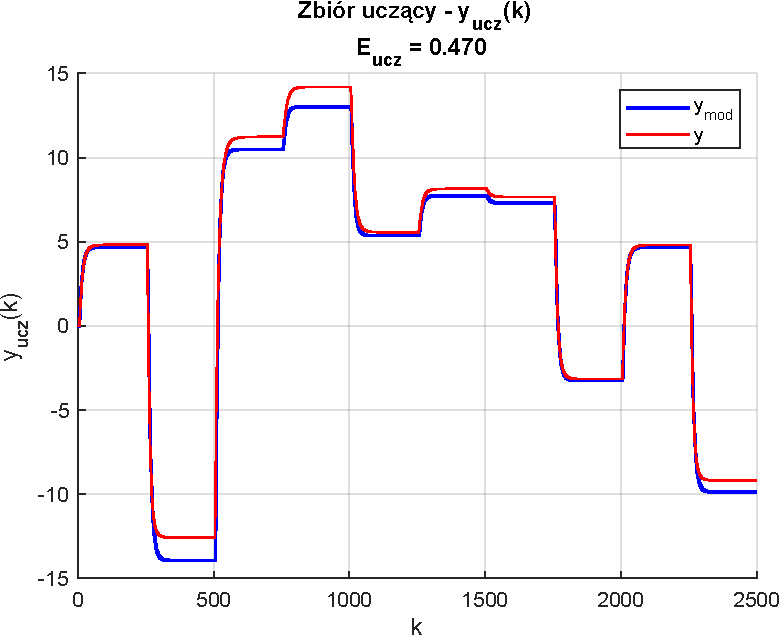
\includegraphics[width=0.45\textwidth]{pictures/oe_ucz}}
\hfill
\subfloat[Zbiór weryfikujący.]{
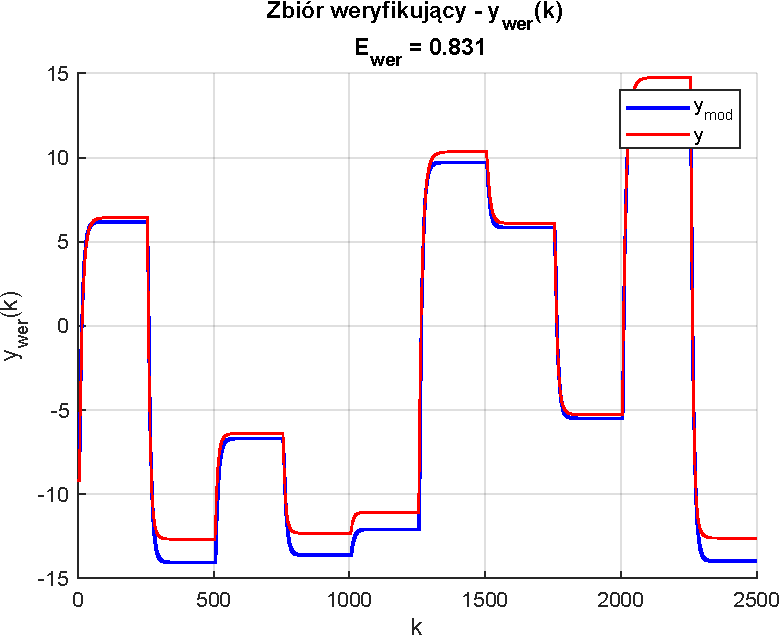
\includegraphics[width=0.45\textwidth]{pictures/oe_wer}}
\caption{Symulacja odpowiednich modeli z wykorzystaniem wygenerowanej sekwencji sygnału sterującego.}
\end{figure}

\newpage

\section{Podejście inżynierskie}
Od tej pory do dalszej analizy postanowiono przyjąć model szarej skrzynki. Informacją o obiekcie był fakt, że układ był inercyjny. Zadano więc wymuszenie w postaci skoku jednostkowego i starano się aproksymować odpowiedź układu dobierając odpowiednie parametru dla modelu transmitancji \textit{First Order Plus Dead Time} (FOPDT), który wyraża się wzorem:

\begin{equation}
G(s) = \frac{K_0e^{-sT_0}}{T_1s + 1}
\end{equation}

\noindent Dobrane parametry:

\begin{equation}
K_0 = \num{0.6025} \hspace{1cm} T_0 = 100 \hspace{1cm} T_1 = 225
\end{equation}

\begin{figure}[h!]
\centering
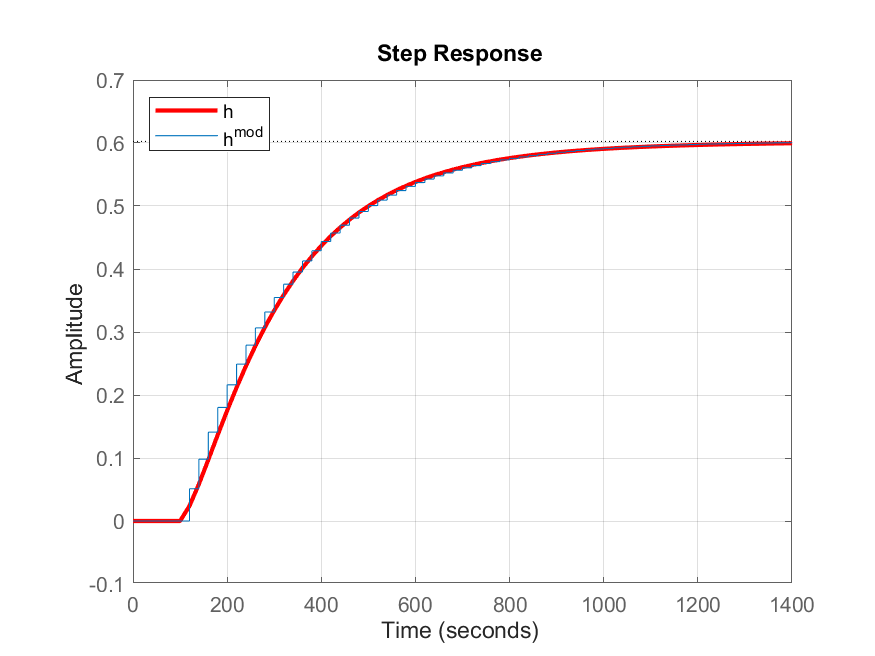
\includegraphics[width=\textwidth]{pictures/model_fopdt}
\caption{Aproksymacja odpowiedzi skokowej układu modelem FOPDT.}
\end{figure}

\newpage

Uzyskany rezultat nie był satysfakcjonujący stąd przyjęto model \textit{Second Order Plus Dead Time} (SOPDT), tj.

\begin{equation}
G(s) = \frac{K_0e^{-sT_0}}{(T_1s + 1)(T_2s + 1)}
\end{equation}

\noindent Dobrane parametry:

\begin{equation}
K_0 = \num{0.6025} \hspace{1cm} T_0 = 100 \hspace{1cm} T_1 = 212 \hspace{1cm} T_2 = 15
\end{equation}

\noindent Wynik prezentował się następująco:

\begin{figure}[h!]
\centering
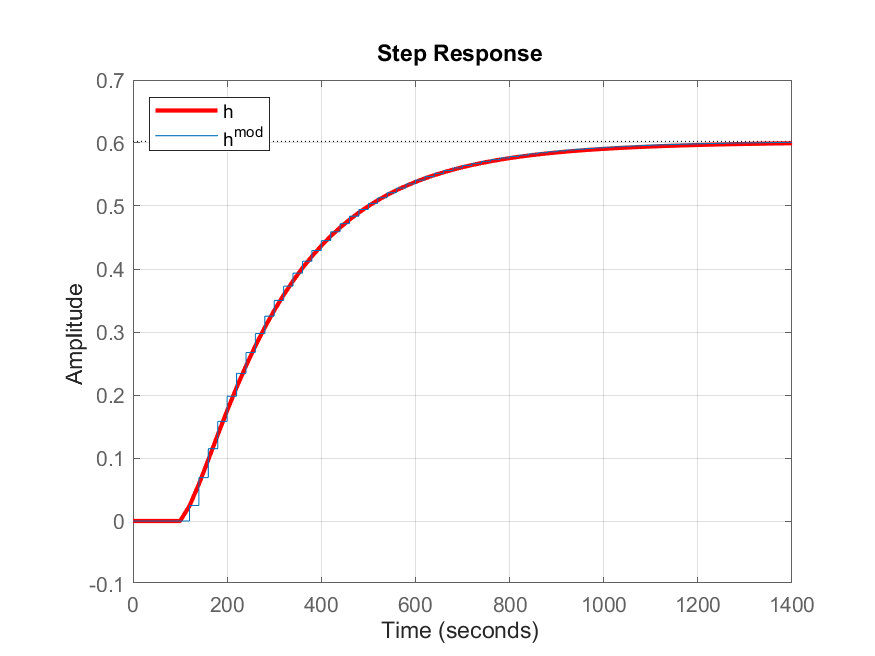
\includegraphics[width=\textwidth]{pictures/model_sopdt}
\caption{Aproksymacja odpowiedzi skokowej układu modelem SOPDT.}
\end{figure}

\newpage

Ponownie, chcąc sprawdzić skuteczność aproksymacji obiektu regulacji wygenerowanym modelem, którego równanie różnicowe jest postaci:

\begin{equation}
\begin{aligned}
y(k) = \num{1.174} y(k-1) - \num{0.2399} y(k-2) + &\num{0.02459} u_1(k-6) + \num{0.01536} u_1(k-7) \\ 
+&\num{0.02459} u_2(k-1) + \num{0.01536} u_2(k-2) 
\end{aligned}
\label{diff_eq}
\end{equation}

\noindent wygenerowano sekwencję sygnału sterującego $u_1(k)$ oraz $u_2(k)$, który są przyrostami wartości sterujących odpowiednio $F_1$ oraz $F_D$.

\begin{figure}[h!]
\begin{center}
\Large \textbf{Model ARX}
\end{center} 
\centering
\subfloat[Zbiór uczący.]{
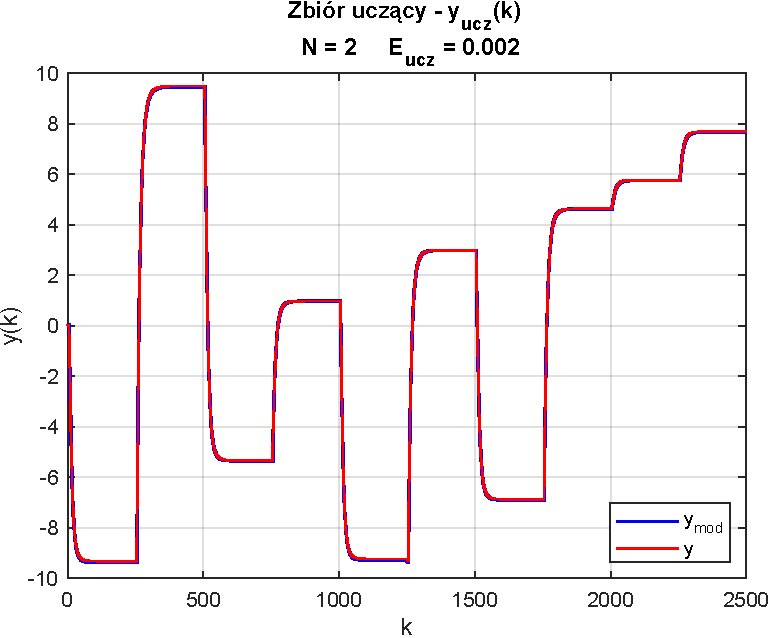
\includegraphics[width=0.45\textwidth]{pictures/arx_ucz_sopdt}}
\hfill
\subfloat[Zbiór weryfikujący.]{
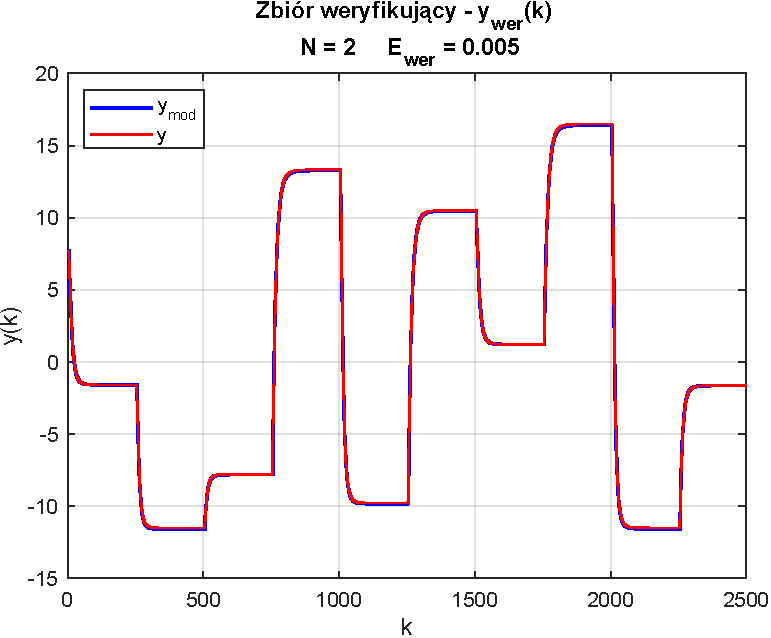
\includegraphics[width=0.45\textwidth]{pictures/arx_wer_sopdt}}

\begin{center}
\Large \textbf{Model OE}
\end{center} 
\subfloat[Zbiór uczący.]{
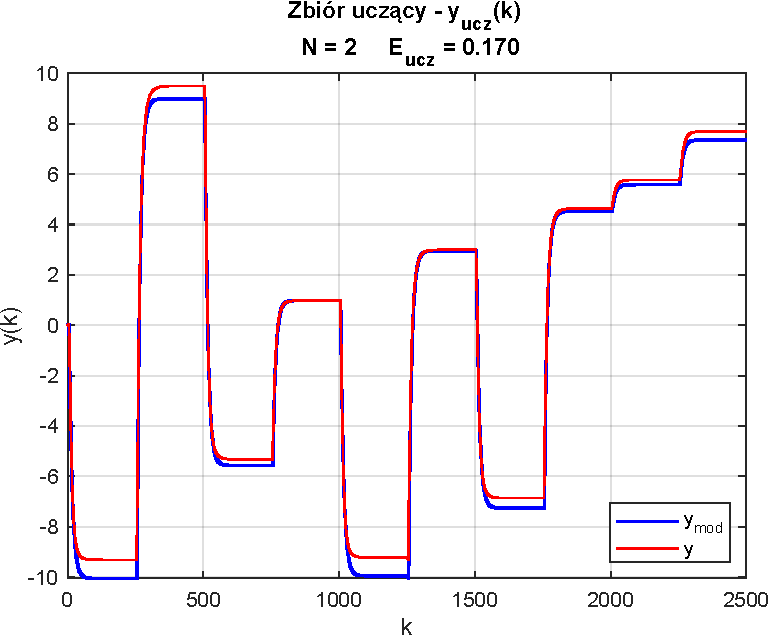
\includegraphics[width=0.45\textwidth]{pictures/oe_ucz_sopdt}}
\hfill
\subfloat[Zbiór weryfikujący.]{
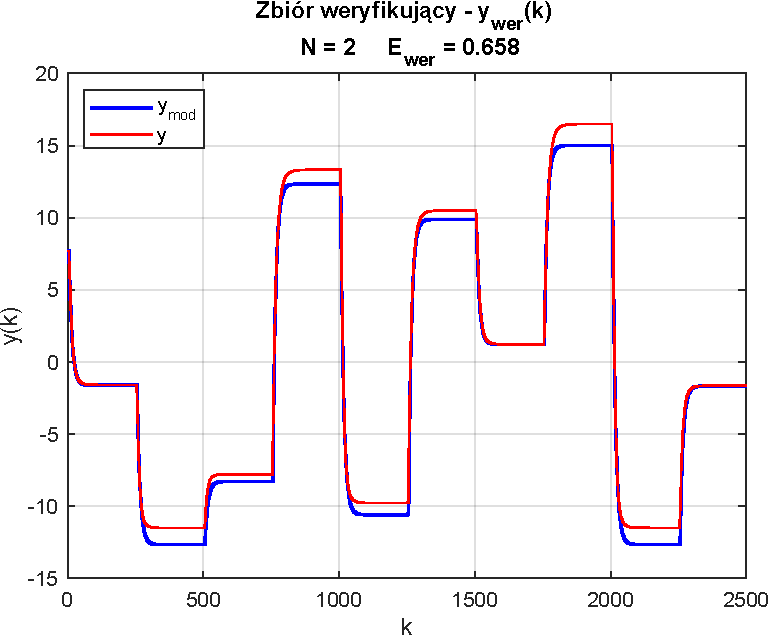
\includegraphics[width=0.45\textwidth]{pictures/oe_wer_sopdt}}
\caption{Symulacja odpowiednich modeli z wykorzystaniem wygenerowanej sekwencji sygnału sterującego.}
\end{figure}

Błędy uznano za akceptowalne na tym poziomie identyfikacji i przyjęto wyznaczony model do dalszej analizy.

\chapter{Model Hammersteina}
W przypadku modelu Hammersteina istota polega na rozdzieleniu dynamiki i statyki w sposób przedstawiony na rys. \ref{hamm_model}.

\begin{figure}[h!]
\centering
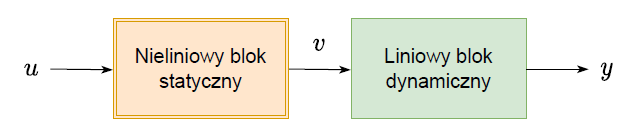
\includegraphics[width=\textwidth]{pictures/hamm_model}
\caption{Reprezentacja graficzna modelu Hammersteina.}
\label{hamm_model}
\end{figure}

\noindent Zatem sygnał sterujący trafia na blok nieliniowej statyki, gdzie jest przekonwertowany na sygnał $z = f(u)$, który następnie trafia na liniowy bloczek dynamiczny. 

\section{Nieliniowy blok statyczny}
Nieliniowość w charakterystyce statycznej została wprowadzono za pomocą logiki rozmytej (ang. \textit{fuzzy logic}), a konkretnie za pomocą modeli rozmytych Takagi-Sugeno. Zastosowano dwa podejścia, jedno standardowe z następnikami liniowymi, natomiast drugie z następnikami hiperbolicznymi.

\section{Następniki liniowe}
Zaczęto od rozmycia zmiennej wejściowej. Symulacyjnie wyznaczono odpowiednią liczbę zbiorów - w tym przypadku pięć.

\begin{figure}[h!]
\centering
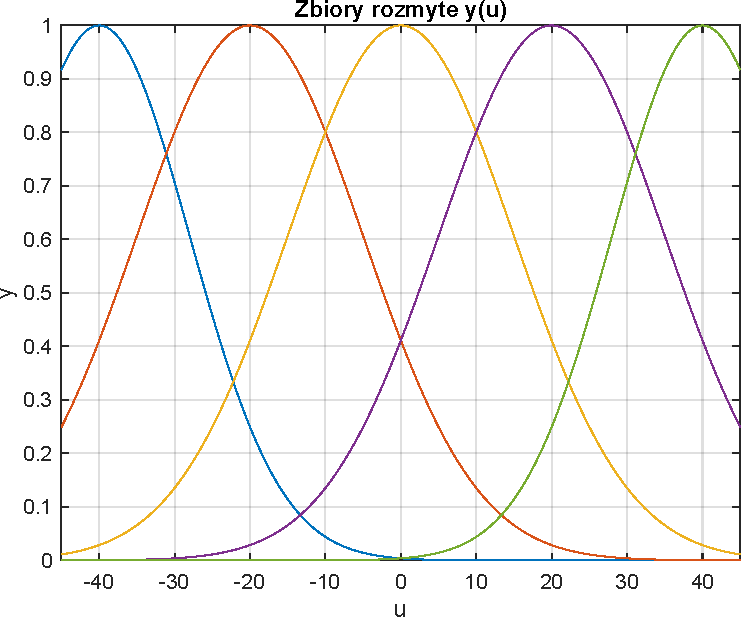
\includegraphics[width=0.5\textwidth]{pictures/fuzzy_set_ham}
\caption{Zbiory rozmyte.}
\label{hamm_model}
\end{figure}

\noindent Zastosowano następniki liniowe postaci:
\begin{equation}
\begin{aligned}
\text{Reguła 1: Jeśli} \quad u^1(k) \quad \text{jest} \quad &U_1, \quad \text{to}: \quad y^1(k) = a_1 + b_1 u^1(k) \\
\text{Reguła 2: Jeśli} \quad u^2(k) \quad \text{jest} \quad &U_2, \quad \text{to}: \quad y^2(k) = a_2 + b_2 u^2(k) \\ 
&\vdots \\
\text{Reguła 5: Jeśli} \quad u^5(k) \quad \text{jest} \quad &U_5, \quad \text{to}: \quad y^2(k) = a_5 + b_5 u^5(k) \\
\end{aligned}
\label{nastepniki_lin}
\end{equation}

Współczynniki w pierwszej iteracji dobierane były poprzez rozwiązanie nieliniowego zadania optymalizacji. W tym celu skorzystano z dostępnych funkcji programu MATLAB, tj. \verb+fminsearch()+, gdzie minimalizowaną funkcją był kwadrat różnicy wyjść wyznaczonej analitycznie charakterystyki statycznej i wyznaczanej charakterystyki rozmytej. Dane statyczne podzielono na zbiory uczący i weryfikujący z tą różnicą - w porównaniu do danych dynamicznych - że wzięto co drugą próbkę do każdego ze zbiorów. Dokładność aproksymacji charakterystyki statycznej przedstawiono na rys. \ref{static_hamm}, natomiast uzyskane błędy były na poziomie $\num{0.001}$. 

\begin{figure}[h!]
\centering
\subfloat[Zbiór uczący.]{
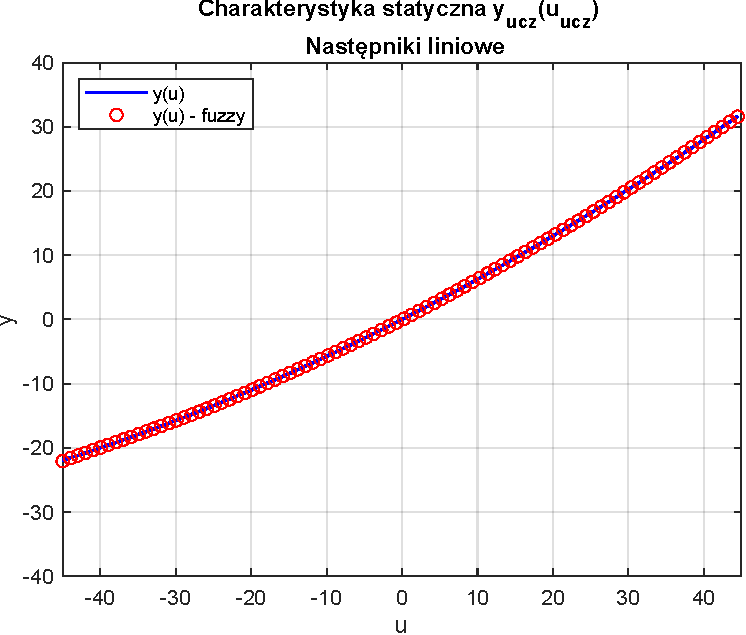
\includegraphics[width=0.45\textwidth]{pictures/static_char_ham_lin_ucz}}
\hfill
\subfloat[Zbiór weryfikujący]{
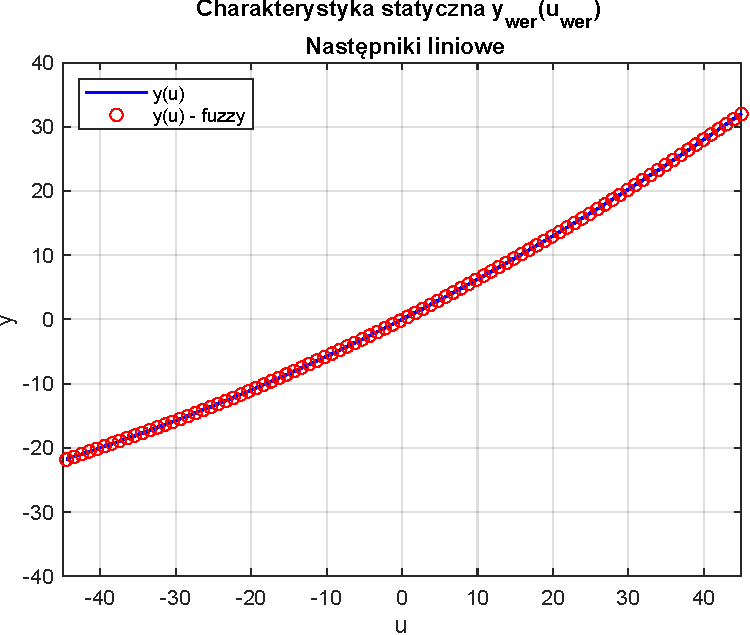
\includegraphics[width=0.45\textwidth]{pictures/static_char_ham_lin_wer}}
\caption{Aproksymacja charakterystyki statycznej przez model rozmyty.}
\label{static_hamm}
\end{figure}

Następnie korzystając z wcześniej opracowanego modelu dynamicznego wykonano szereg symulacji, sprawdzając jak zachowuje się układ w zależności od losowo wygenerowanych sygnałów sterujących. Efekty symulacji przedstawiono poniżej.

%%%%%%%%%%%%%%%%%%%%%% PIERWSZA SEKWENCJA %%%%%%%%%%%%%%%%%%%%%%

\begin{figure}[p!]

\begin{center}
\Large \textbf{I sekwencja} \\
\vspace{0.5cm}
\Large \textbf{Model dynamiczny}
\end{center}

\centering
\subfloat[Zbiór uczący.]{
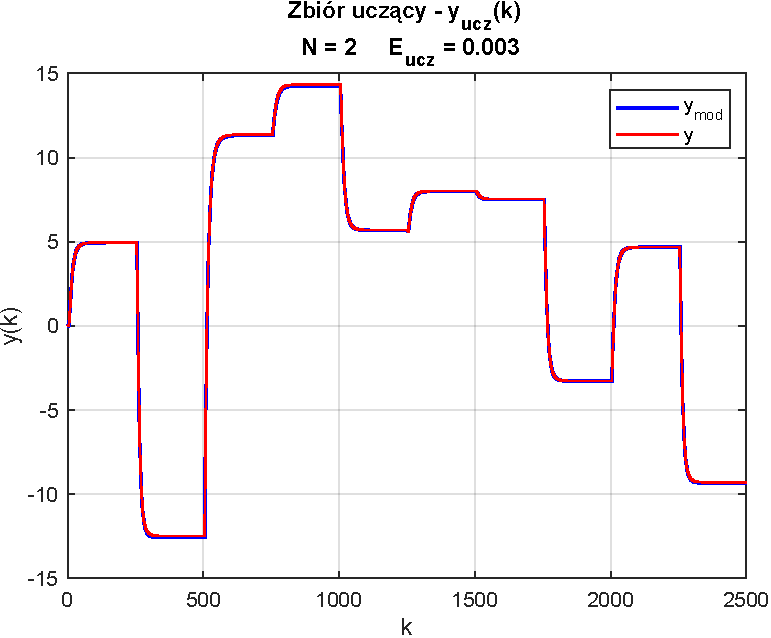
\includegraphics[width=0.45\textwidth]{pictures/arx_ucz_1}}
\hfill
\subfloat[Zbiór weryfikujący]{
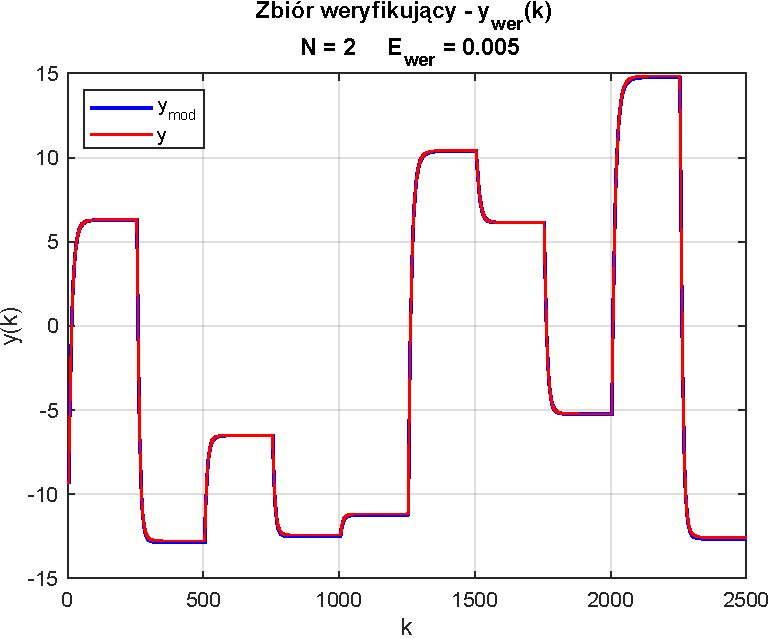
\includegraphics[width=0.45\textwidth]{pictures/arx_wer_1}}

\begin{center}
\Large \textbf{Model Hammersteina}
\end{center}

\subfloat[Zbiór uczący.]{
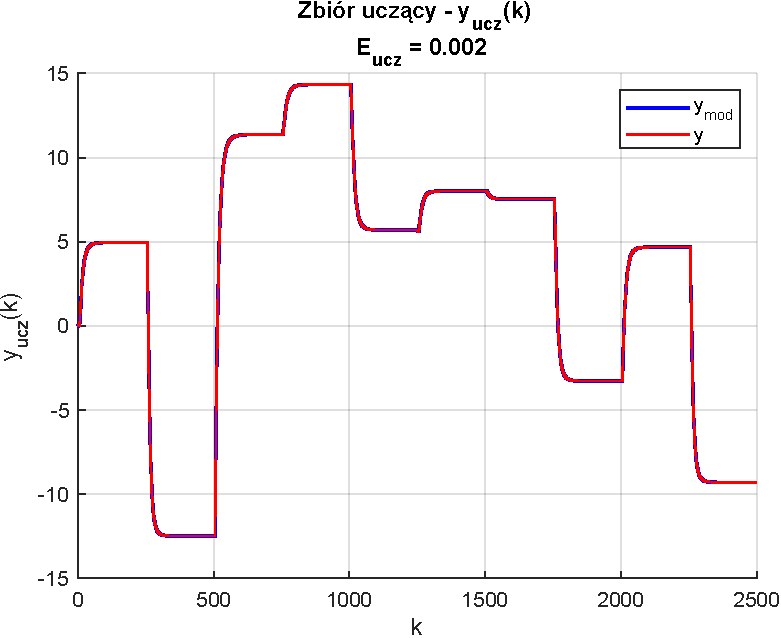
\includegraphics[width=0.45\textwidth]{pictures/arx_hamm_ucz_1}}
\hfill
\subfloat[Zbiór weryfikujący]{
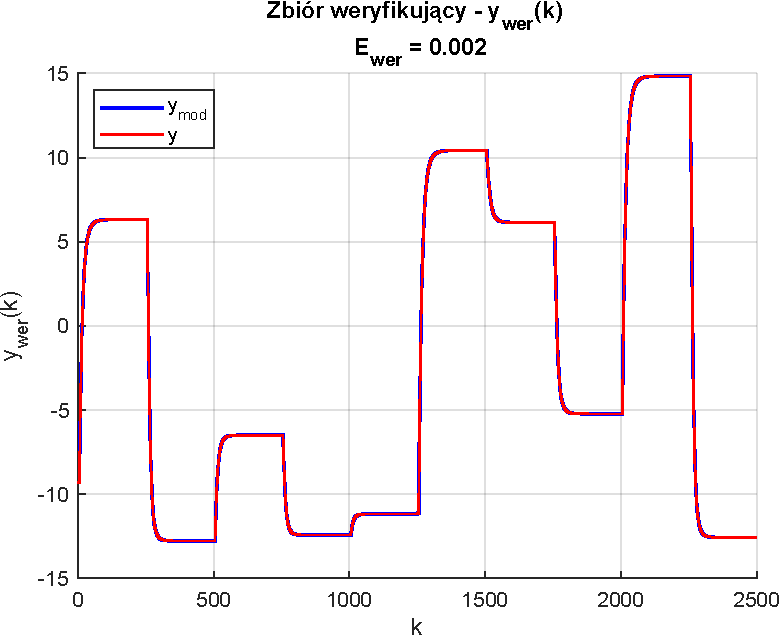
\includegraphics[width=0.45\textwidth]{pictures/arx_hamm_wer_1}}
\caption{Porównanie przebiegu sygnału wyjściowego modelu dynamicznego i modelu Hammesteina w trybie bez rekurencji.}
\end{figure}

\begin{figure}[p!]

\begin{center}
\Large \textbf{I sekwencja} \\
\vspace{0.5cm}
\Large \textbf{Model dynamiczny}
\end{center}

\centering
\subfloat[Zbiór uczący.]{
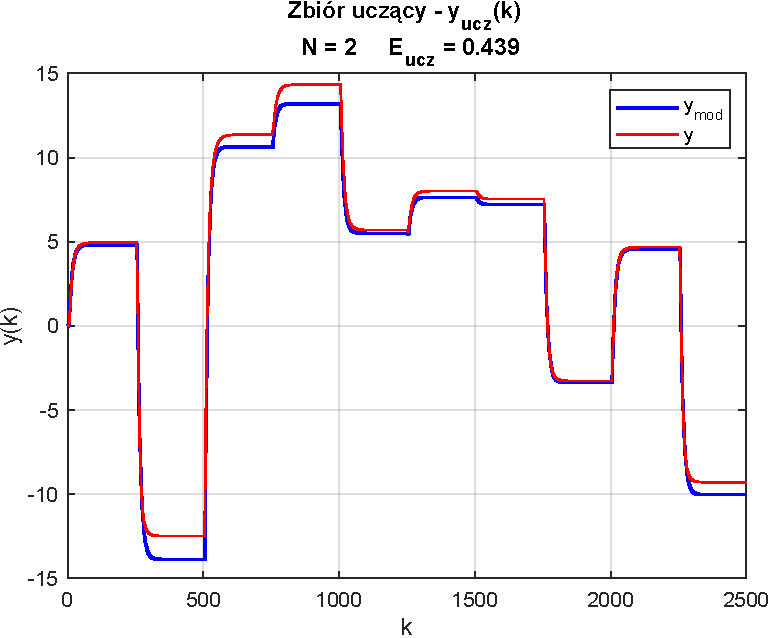
\includegraphics[width=0.45\textwidth]{pictures/oe_ucz_1}}
\hfill
\subfloat[Zbiór weryfikujący]{
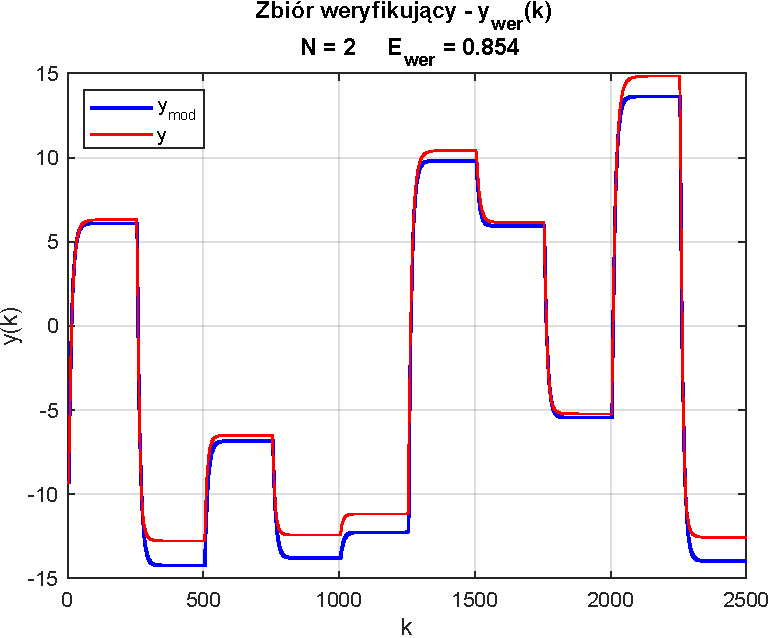
\includegraphics[width=0.45\textwidth]{pictures/oe_wer_1}}

\begin{center}
\Large \textbf{Model Hammersteina}
\end{center}

\subfloat[Zbiór uczący.]{
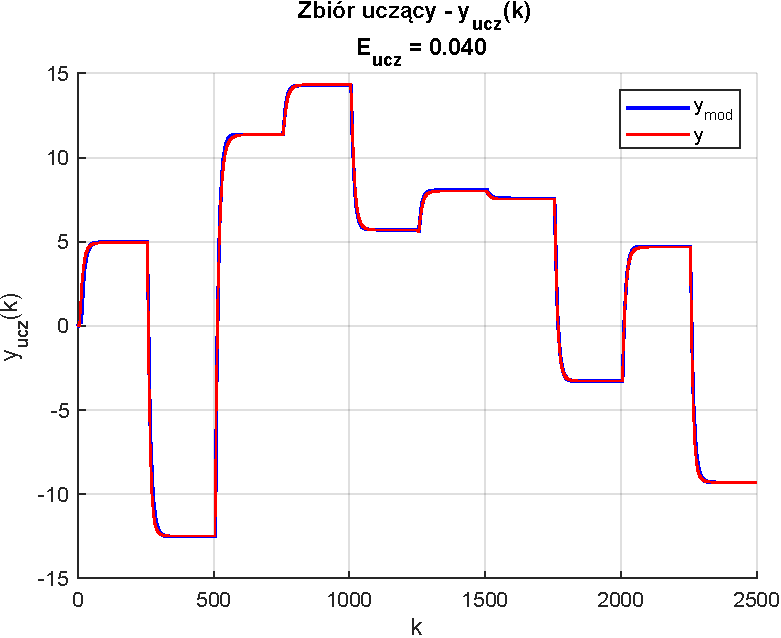
\includegraphics[width=0.45\textwidth]{pictures/oe_hamm_ucz_1}}
\hfill
\subfloat[Zbiór weryfikujący]{
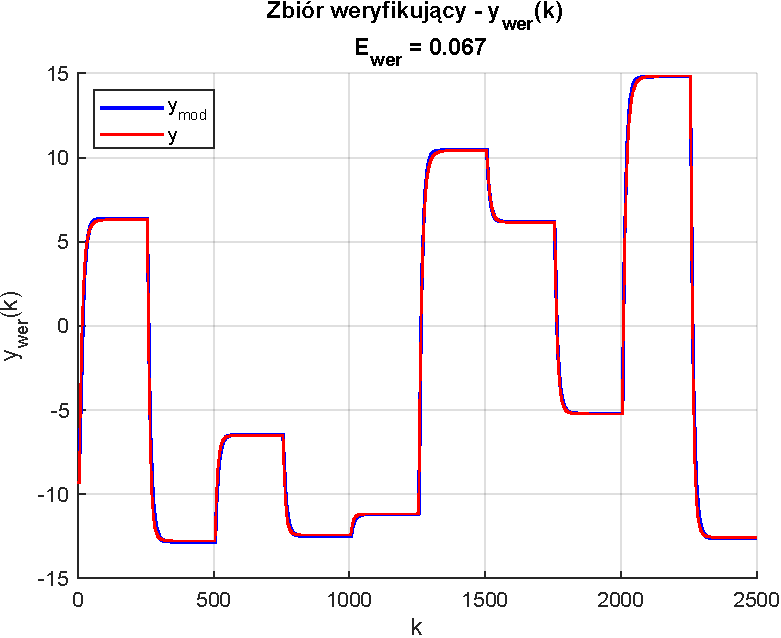
\includegraphics[width=0.45\textwidth]{pictures/oe_hamm_wer_1}}
\caption{Porównanie przebiegu sygnału wyjściowego modelu dynamicznego i modelu Hammesteina w trybie z rekurencją.}
\end{figure}

%%%%%%%%%%%%%%%%%%%%%% DRUGA SEKWENCJA %%%%%%%%%%%%%%%%%%%%%%

\begin{figure}[p!]

\begin{center}
\Large \textbf{II sekwencja} \\
\vspace{0.5cm}
\Large \textbf{Model dynamiczny}
\end{center}

\centering
\subfloat[Zbiór uczący.]{
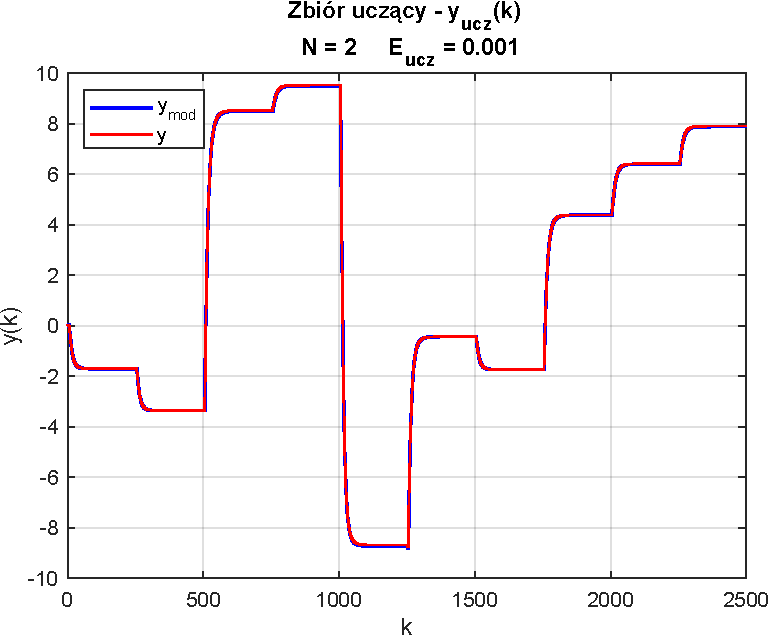
\includegraphics[width=0.45\textwidth]{pictures/arx_ucz_2}}
\hfill
\subfloat[Zbiór weryfikujący]{
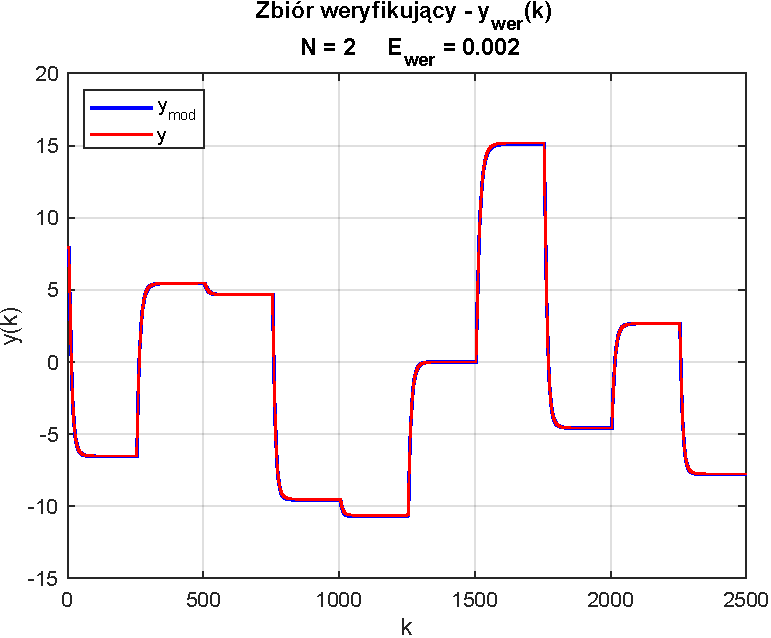
\includegraphics[width=0.45\textwidth]{pictures/arx_wer_2}}

\begin{center}
\Large \textbf{Model Hammersteina}
\end{center}

\subfloat[Zbiór uczący.]{
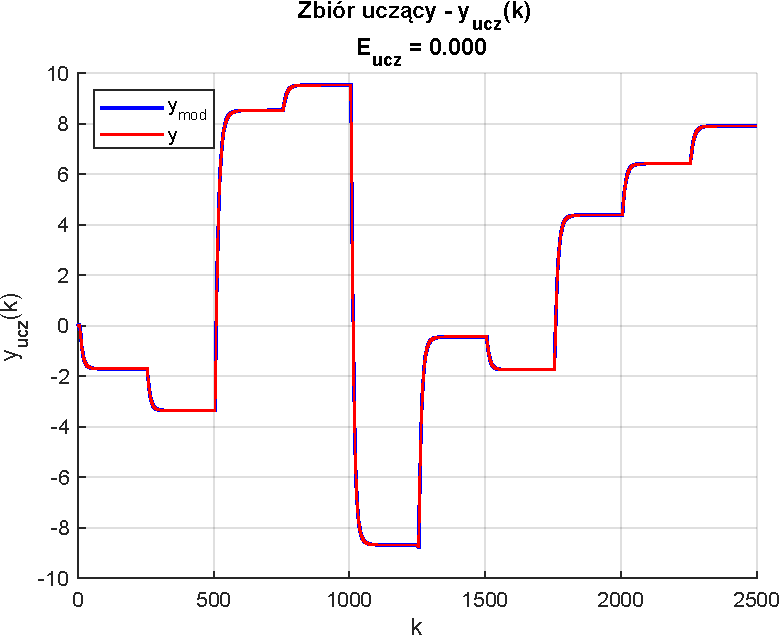
\includegraphics[width=0.45\textwidth]{pictures/arx_hamm_ucz_2}}
\hfill
\subfloat[Zbiór weryfikujący]{
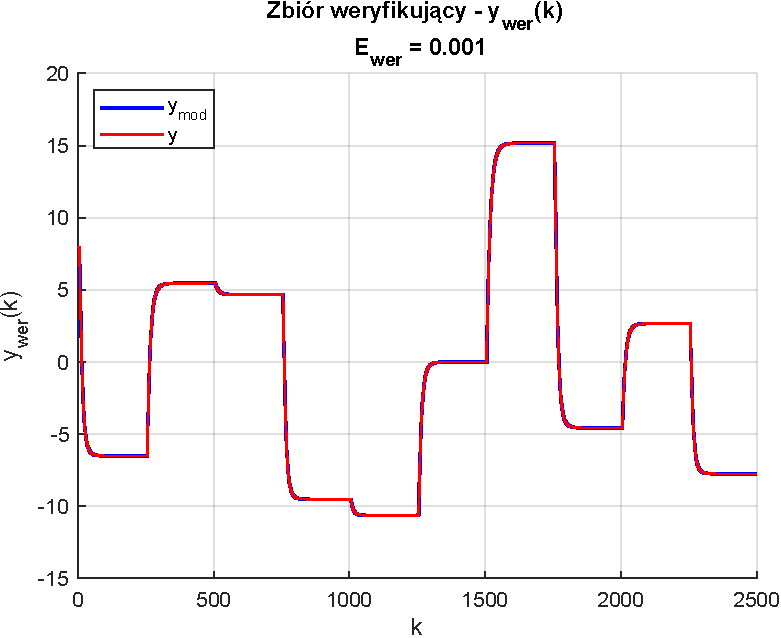
\includegraphics[width=0.45\textwidth]{pictures/arx_hamm_wer_2}}
\caption{Porównanie przebiegu sygnału wyjściowego modelu dynamicznego i modelu Hammesteina w trybie bez rekurencji.}
\end{figure}

\begin{figure}[p!]

\begin{center}
\Large \textbf{II sekwencja} \\
\vspace{0.5cm}
\Large \textbf{Model dynamiczny}
\end{center}

\centering
\subfloat[Zbiór uczący.]{
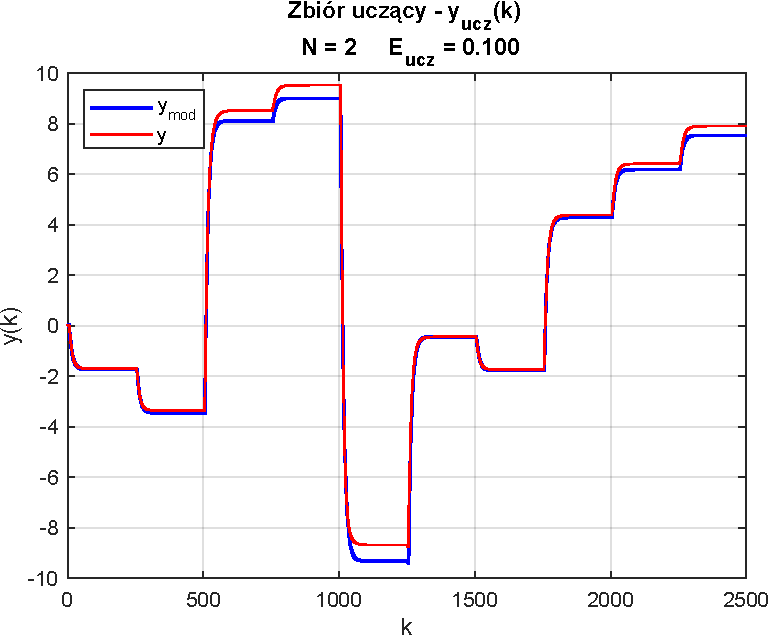
\includegraphics[width=0.45\textwidth]{pictures/oe_ucz_2}}
\hfill
\subfloat[Zbiór weryfikujący]{
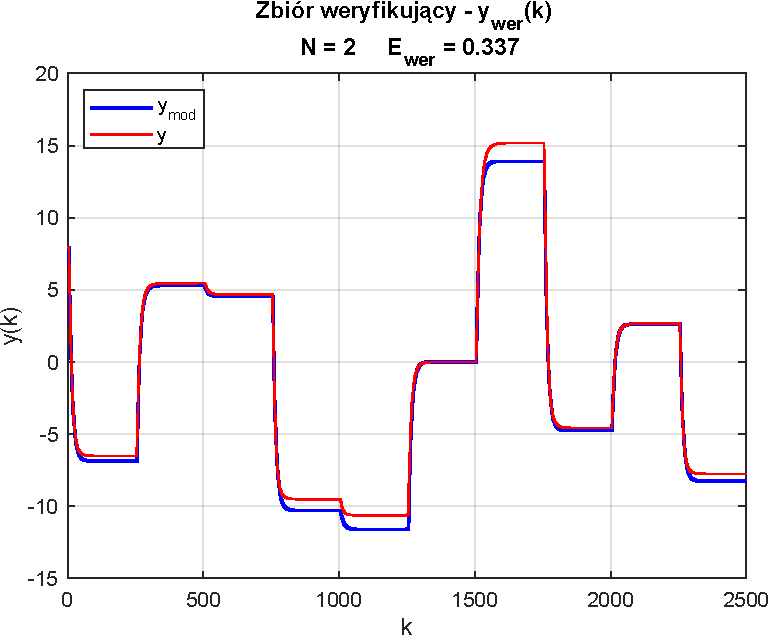
\includegraphics[width=0.45\textwidth]{pictures/oe_wer_2}}

\begin{center}
\Large \textbf{Model Hammersteina}
\end{center}

\subfloat[Zbiór uczący.]{
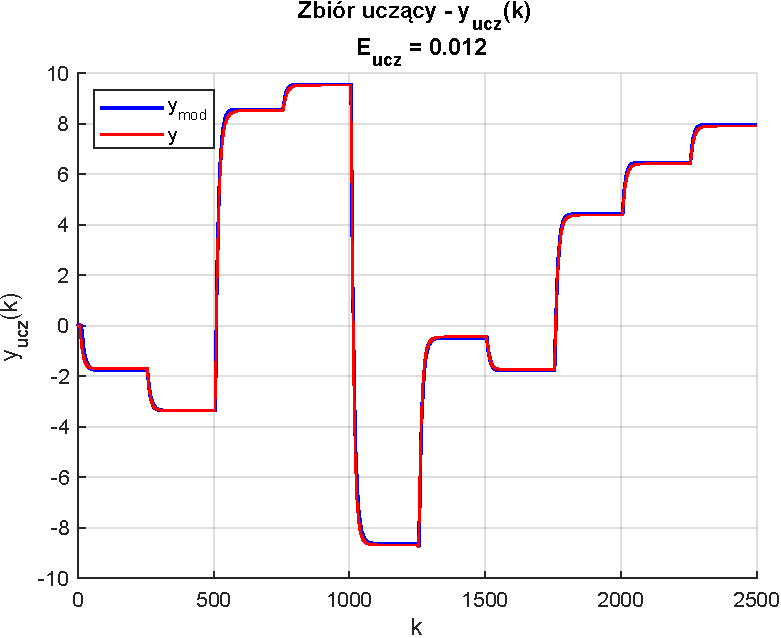
\includegraphics[width=0.45\textwidth]{pictures/oe_hamm_ucz_2}}
\hfill
\subfloat[Zbiór weryfikujący]{
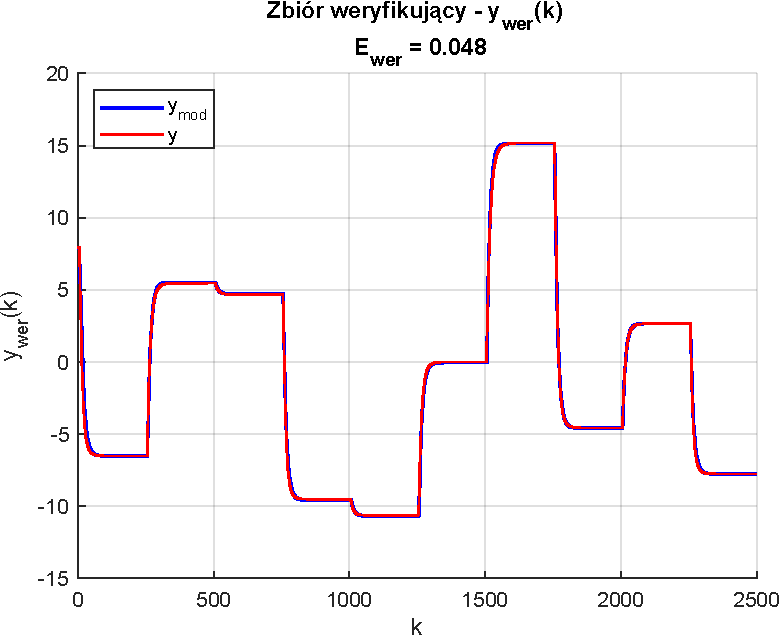
\includegraphics[width=0.45\textwidth]{pictures/oe_hamm_wer_2}}
\caption{Porównanie przebiegu sygnału wyjściowego modelu dynamicznego i modelu Hammesteina w trybie z rekurencją.}
\end{figure}

%%%%%%%%%%%%%%%%%%%%%% TRZECIA SEKWENCJA %%%%%%%%%%%%%%%%%%%%%%

\begin{figure}[p!]

\begin{center}
\Large \textbf{III sekwencja} \\
\vspace{0.5cm}
\Large \textbf{Model dynamiczny}
\end{center}

\centering
\subfloat[Zbiór uczący.]{
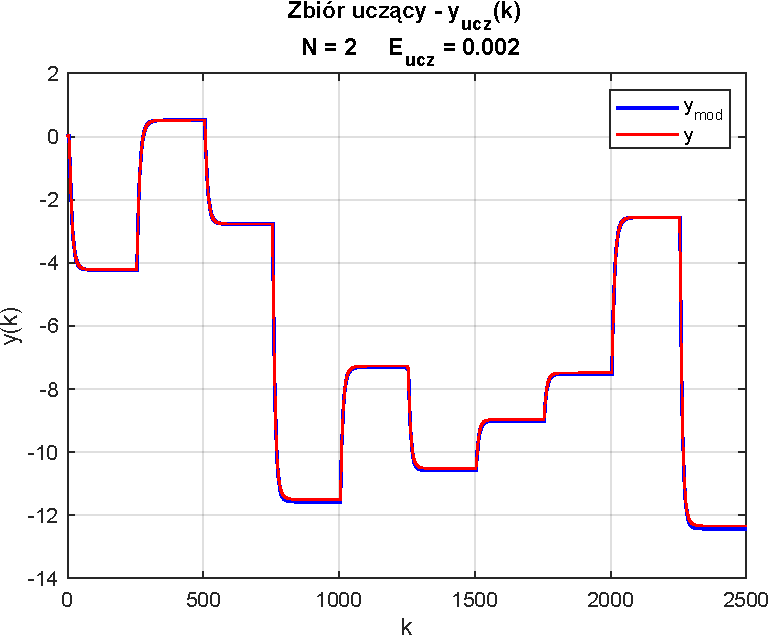
\includegraphics[width=0.45\textwidth]{pictures/arx_ucz_3}}
\hfill
\subfloat[Zbiór weryfikujący]{
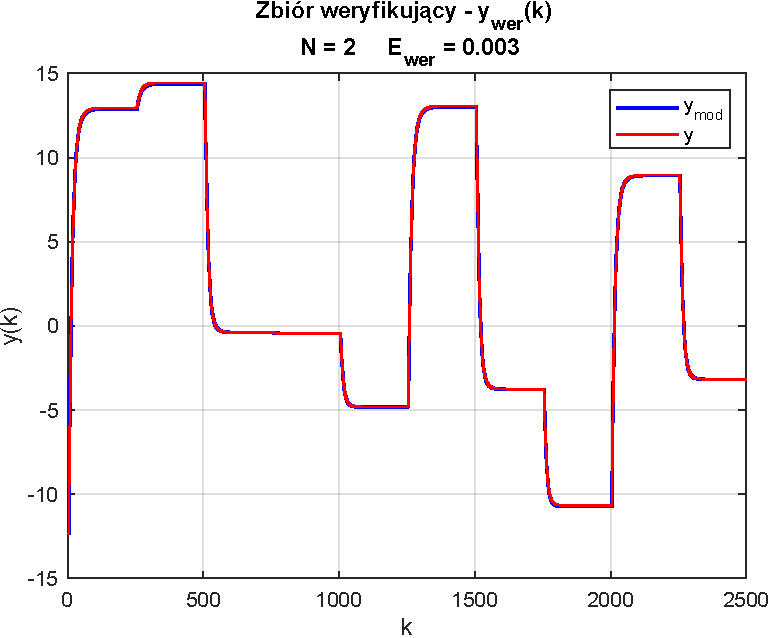
\includegraphics[width=0.45\textwidth]{pictures/arx_wer_3}}

\begin{center}
\Large \textbf{Model Hammersteina}
\end{center}

\subfloat[Zbiór uczący.]{
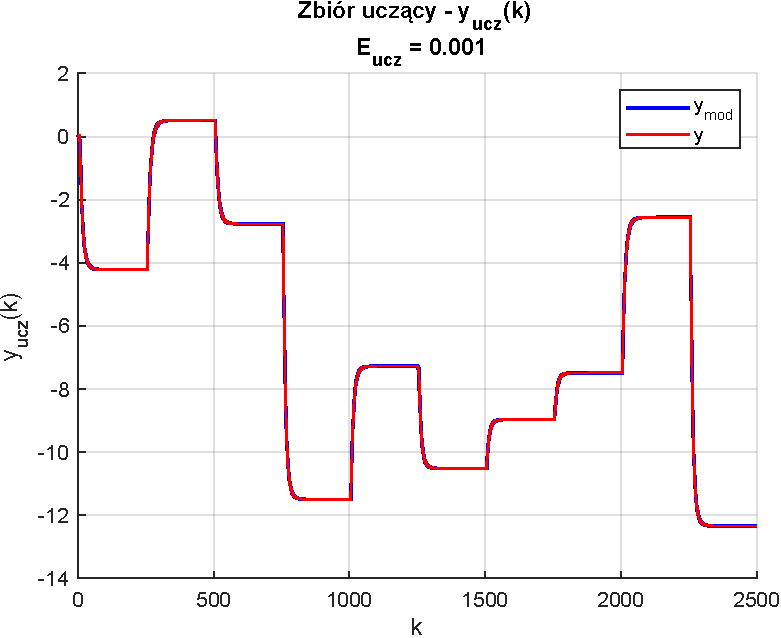
\includegraphics[width=0.45\textwidth]{pictures/arx_hamm_ucz_3}}
\hfill
\subfloat[Zbiór weryfikujący]{
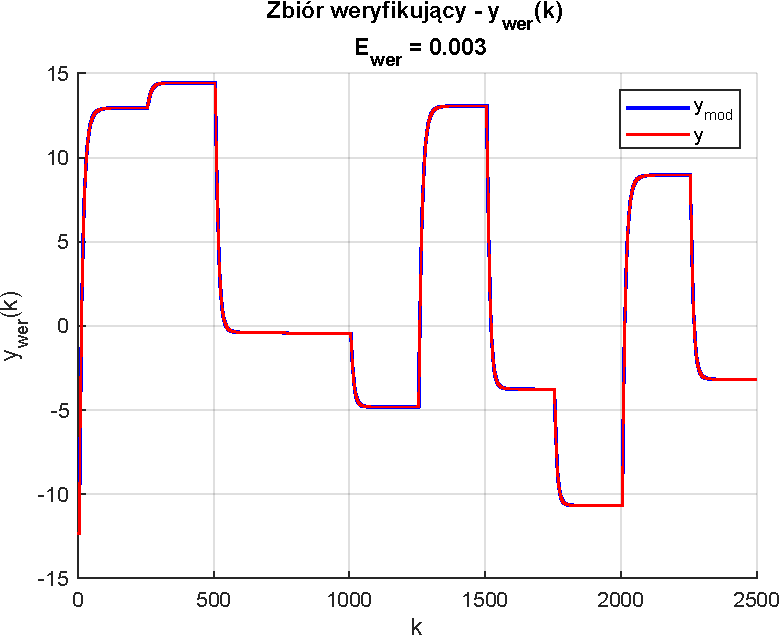
\includegraphics[width=0.45\textwidth]{pictures/arx_hamm_wer_3}}
\caption{Porównanie przebiegu sygnału wyjściowego modelu dynamicznego i modelu Hammesteina w trybie bez rekurencji.}
\end{figure}

\newpage

\begin{figure}[h!]

\begin{center}
\Large \textbf{III sekwencja} \\
\vspace{0.5cm}
\Large \textbf{Model dynamiczny}
\end{center}

\centering
\subfloat[Zbiór uczący.]{
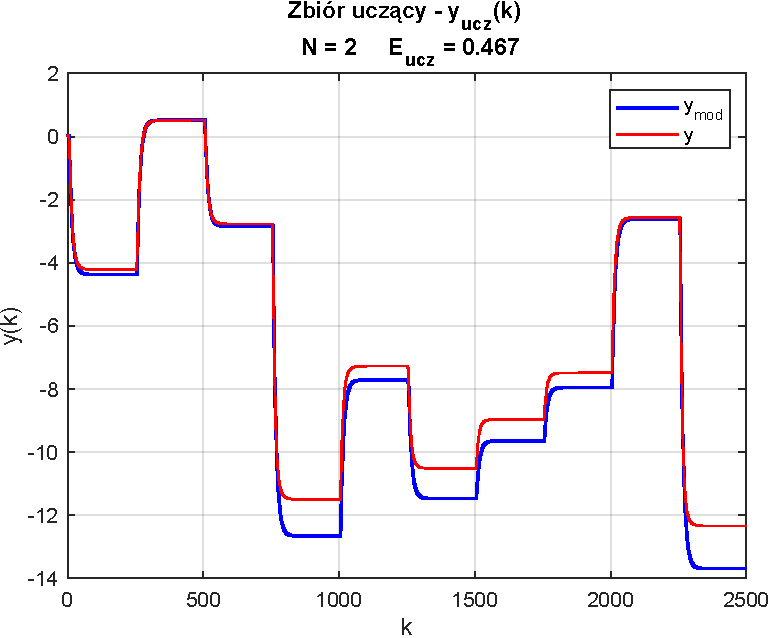
\includegraphics[width=0.45\textwidth]{pictures/oe_ucz_3}}
\hfill
\subfloat[Zbiór weryfikujący]{
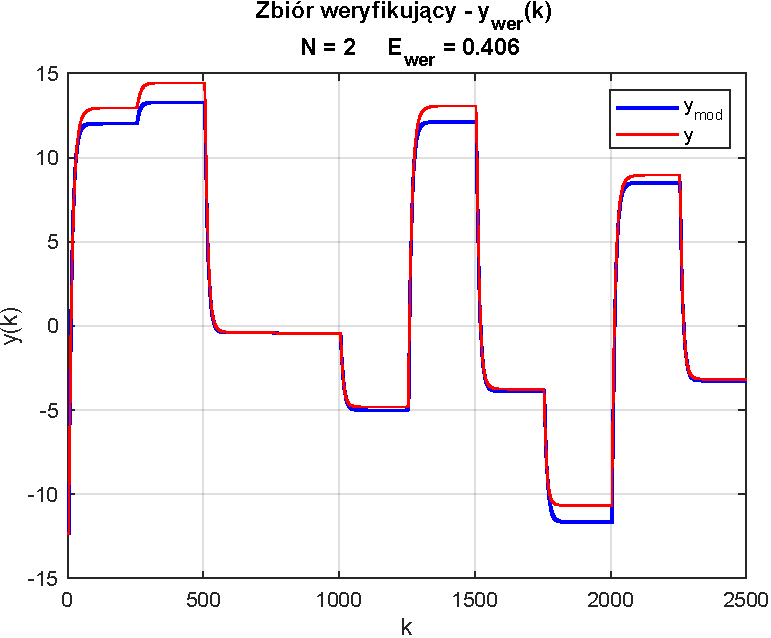
\includegraphics[width=0.45\textwidth]{pictures/oe_wer_3}}

\begin{center}
\Large \textbf{Model Hammersteina}
\end{center}

\subfloat[Zbiór uczący.]{
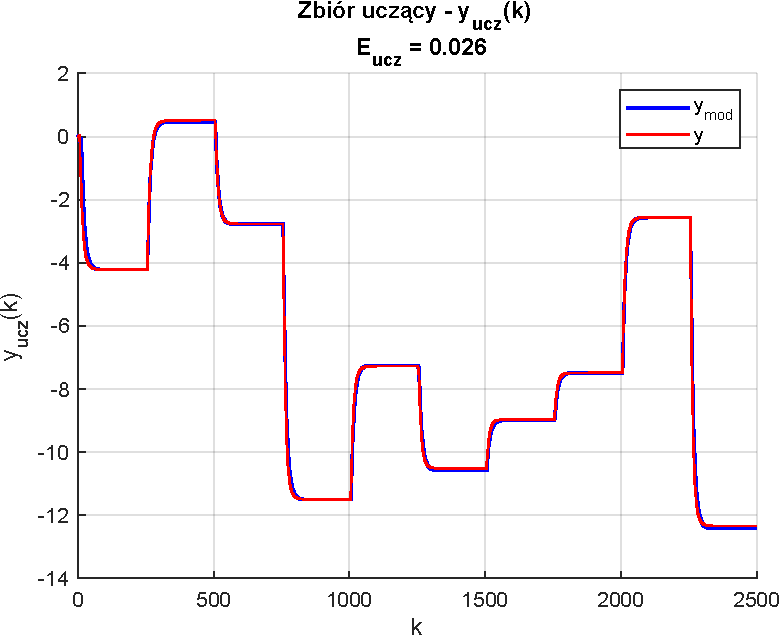
\includegraphics[width=0.45\textwidth]{pictures/oe_hamm_ucz_3}}
\hfill
\subfloat[Zbiór weryfikujący]{
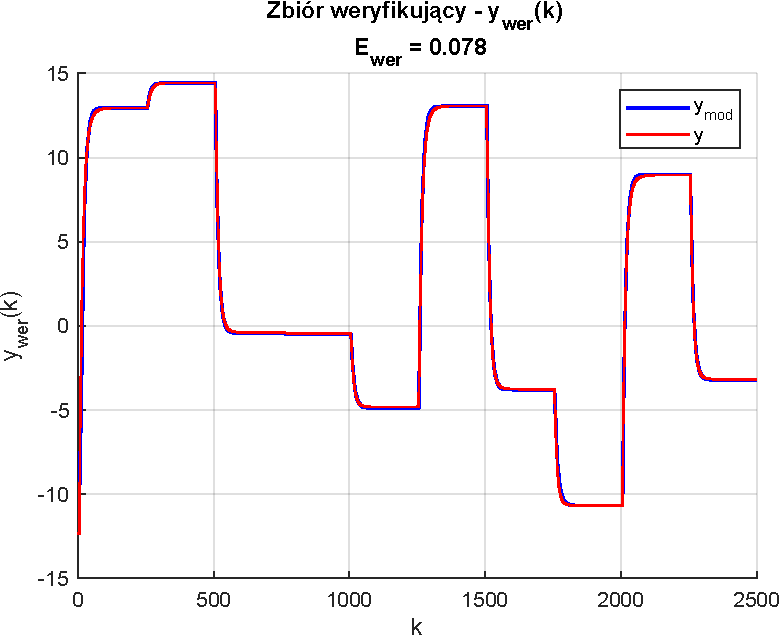
\includegraphics[width=0.45\textwidth]{pictures/oe_hamm_wer_3}}
\caption{Porównanie przebiegu sygnału wyjściowego modelu dynamicznego i modelu Hammesteina w trybie z rekurencją.}
\end{figure}

W każdym z otrzymanych przypadków model Hammersteina z rozmytą statyką i następnikami liniowymi okazywał się być lepszy niż standardowy model dynamiczny, zarówno ten testowany w trybie bez rekurencji, jak i z rekurencją. Istotnie, wprowadzenie nieliniowości do obiektu nieliniowego opisanego liniowym modelem dynamicznym poprawia dokładność otrzymywanych wyników. Jako akceptowalną granicę przyjęto błąd na poziomie $E = \num{0.1}$, a kluczowym przypadkiem był model testowany w trybie rekurencyjnym dla zbioru weryfikującego. Model Hammersteina w tej konfiguracji dawał na tyle satysfakcjonujące wyniki, że postanowiono dalej nie ingerować w dostrajanie współczynników modelu. 

\newpage

\section{Następniki hiperboliczne}

\chapter{Model Wienera}
Istota modelu Wienera jest dokładnie taka sama jak w przypadku modelu Hammersteina z tym, że nieliniową statykę poprzedzono liniową dynamika - odwrotnie niż jak to było w przypadku omówionego modelu.

\begin{figure}[h!]
\centering
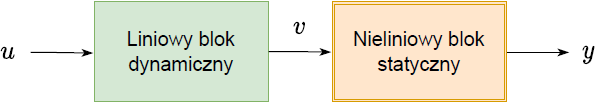
\includegraphics[width=\textwidth]{pictures/wien_model}
\caption{Reprezentacja graficzna modelu Wienera.}
\end{figure}

Sygnał wejściowy trafia na liniowy blok dynamiczny, gdzie jest przekonwertowany na sygnał $v = f(u)$, który trafia na nieliniową statykę, której wyjściem jest sygnał $y$. W przypadku dynamiki skorzystano z wyznaczonego wcześniej modelu dynamicznego (\ref{diff_eq}), natomiast zmianie uległa charakterystyka statyczna.

\section{Następniki liniowe}
W przypadku modelu Wienera aproksymacja charakterystyki statycznej przysporzyła więcej problemów niżeli w przypadku modelu Hammersteina. Przyjęty przedział rozmywania zmiennej $v \in [-25;25]$ podzielono na pięć zbiorów.

\begin{figure}[h!]
\centering
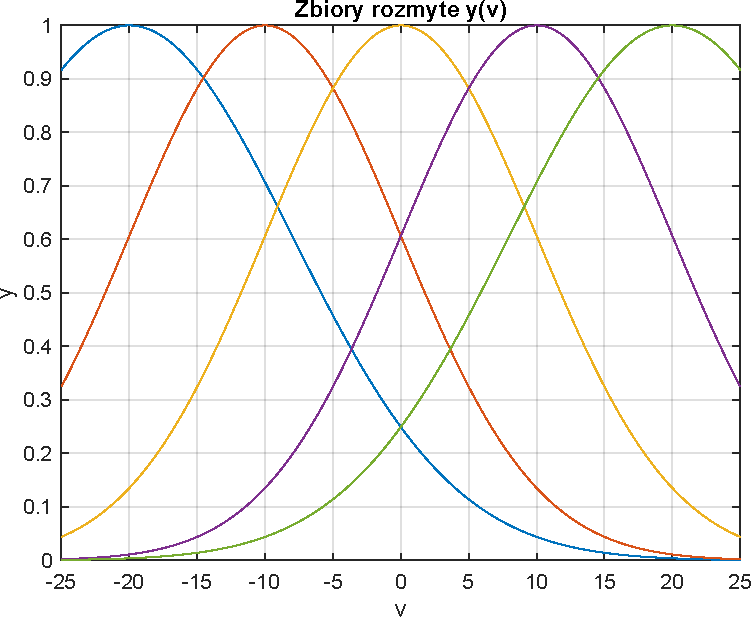
\includegraphics[width=0.6\textwidth]{pictures/fuzzy_set_wien}
\caption{Zbiory rozmyte.}
\end{figure}

\newpage

\noindent Dzięki zastosowanemu podziałowi udało się otrzymać następującą aproksymację charakterystyki statycznej.

\begin{figure}[h!]
\centering
\subfloat[Zbiór uczący.]{
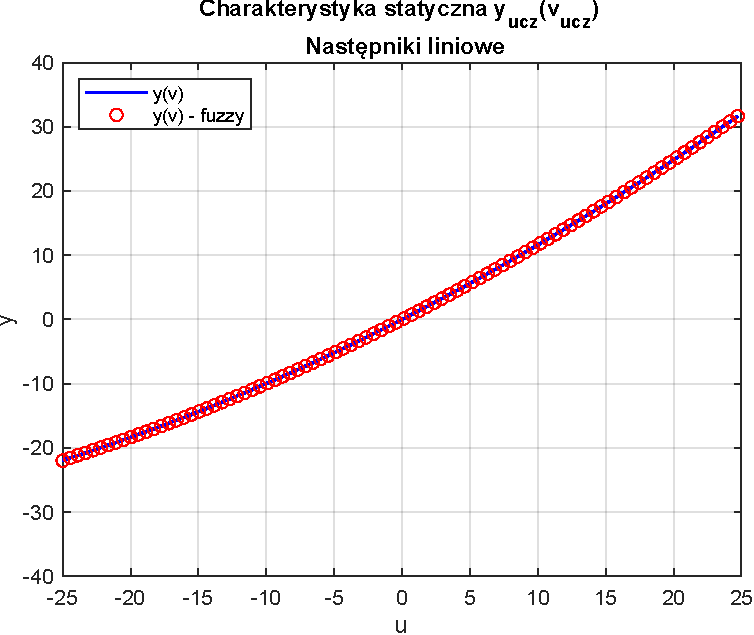
\includegraphics[width=0.45\textwidth]{pictures/static_char_wien_lin_ucz}}
\hfill
\subfloat[Zbiór weryfikujący]{
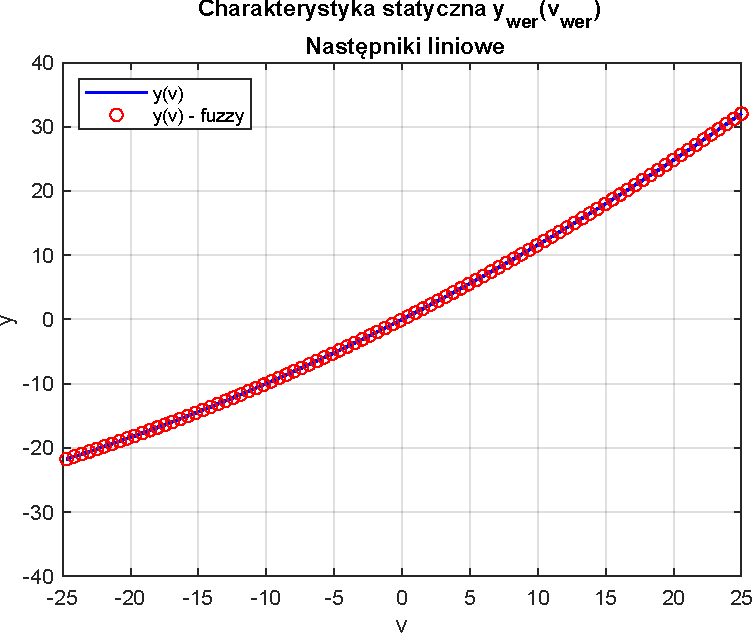
\includegraphics[width=0.45\textwidth]{pictures/static_char_wien_lin_wer}}
\caption{Aproksymacja charakterystyki statycznej przez model rozmyty.}
\end{figure}

Następniki liniowe reguł przybrały postać zaprezentowaną w \ref{nastepniki_lin}. Ponownie pierwsze przybliżenie zostało wyznaczone w za pomocą funkcji MATLAB, tym razem jednak niezbędne okazało się ręczne dostrajanie otrzymanych współczynników. Do problemu zdecydowano podejść w następujący sposób - starano się minimalizować błąd zbioru uczącego, następnie analizowano zachowanie modelu w przypadku zbiory weryfikującego. Wygenerowano kilka sekwencji sygnału sterującego i porównano zachowanie modelu dynamicznego i modelu Wienera.

\newpage

\begin{figure}[h!]

\begin{center}
\Large \textbf{I sekwencja} \\
\vspace{0.5cm}
\Large \textbf{Model dynamiczny}
\end{center}

\centering
\subfloat[Zbiór uczący.]{
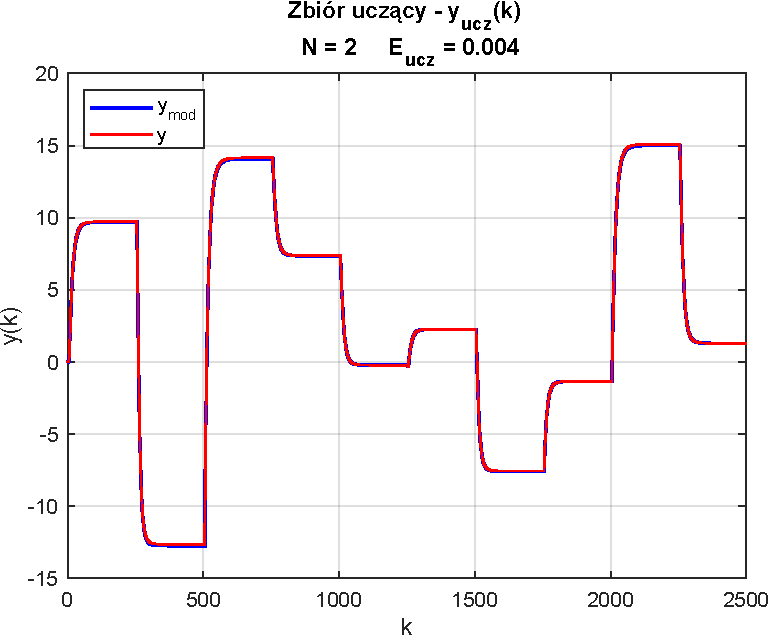
\includegraphics[width=0.45\textwidth]{pictures/arx_ucz_11}}
\hfill
\subfloat[Zbiór weryfikujący]{
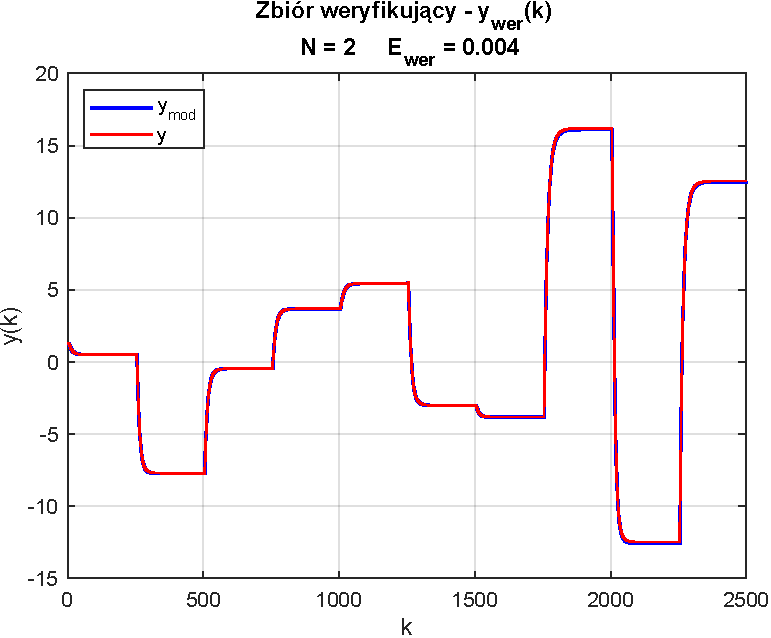
\includegraphics[width=0.45\textwidth]{pictures/arx_wer_11}}

\begin{center}
\Large \textbf{Model Wienera}
\end{center}

\subfloat[Zbiór uczący.]{
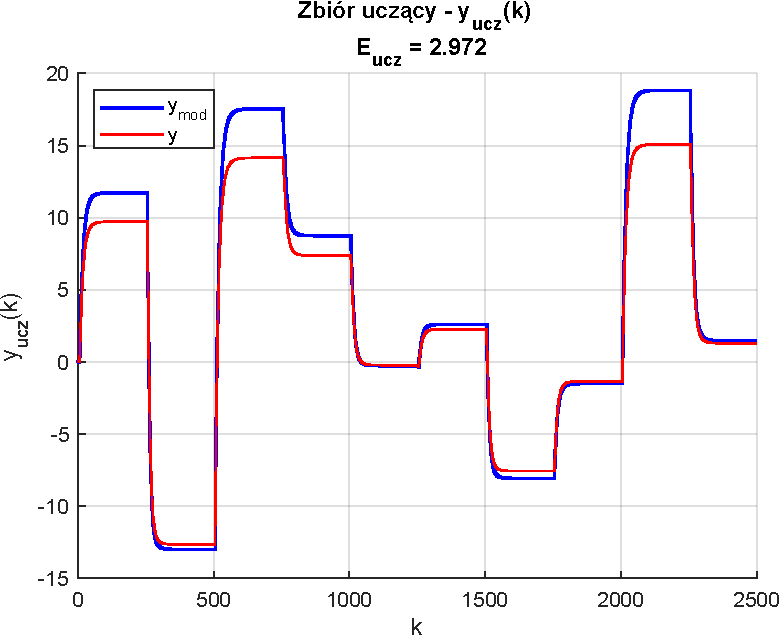
\includegraphics[width=0.45\textwidth]{pictures/arx_wien_ucz_11}}
\hfill
\subfloat[Zbiór weryfikujący]{
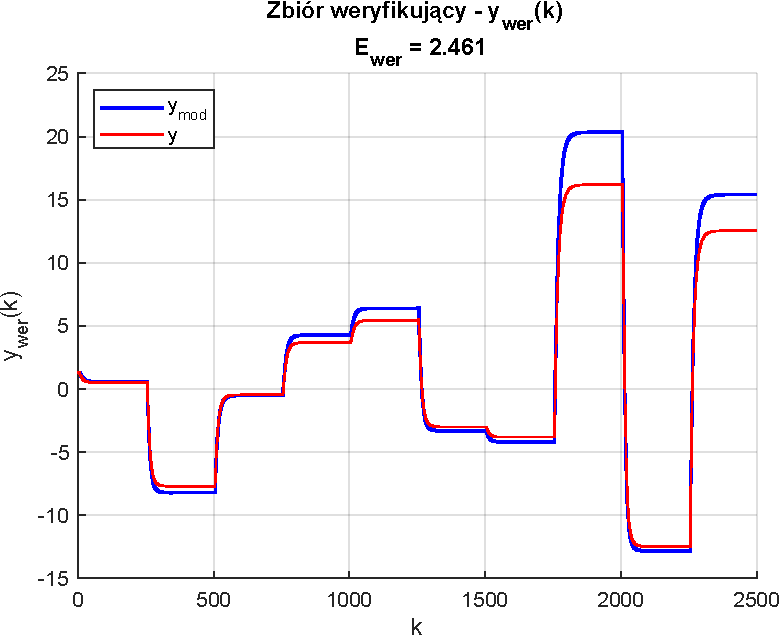
\includegraphics[width=0.45\textwidth]{pictures/arx_wien_wer_11}}
\caption{Porównanie przebiegu sygnału wyjściowego modelu dynamicznego i modelu Wienera w trybie bez rekurencji.}
\end{figure}

Jak widać na powyższych rysunkach dokładność osiągnięta przez model Wienera w trybie ARX jest nieakceptowalna - postanowiono ręcznie dostroić model. Dokonano tego tylko poprzez zmianę wartości współczynników lokalnych modeli systemu rozmytego. Uzyskane rezultaty zaprezentowano na rys. \ref{wien_arx}.

\newpage

\begin{figure}[h!]
\centering
\subfloat[Zbiór uczący.]{
\includegraphics[width=0.7\textwidth]{pictures/arx_wien_ucz_12}}
\vfill
\subfloat[Zbiór weryfikujący]{
\includegraphics[width=0.7\textwidth]{pictures/arx_wien_wer_12}}
\caption{Przebiegu sygnału wyjściowego modelu Wienera w trybie bez rekurencji po dostrojeniu współczynników następników.}
\label{wien_arx}
\end{figure}

Model Wienera po ręcznym strojeniu osiągnął próg akceptowalności w kontekście kryterium jakości - $E = \num{0.1}$. Analogiczne podejście zastosowano w przypadku testowania modelu w trybie rekurencyjnym.

\newpage

\begin{figure}[h!]

\begin{center}
\Large \textbf{I sekwencja} \\
\vspace{0.5cm}
\Large \textbf{Model dynamiczny}
\end{center}

\centering
\subfloat[Zbiór uczący.]{
\includegraphics[width=0.45\textwidth]{pictures/oe_ucz_11}}
\hfill
\subfloat[Zbiór weryfikujący]{
\includegraphics[width=0.45\textwidth]{pictures/oe_wer_11}}

\begin{center}
\Large \textbf{Model Wienera}
\end{center}

\subfloat[Zbiór uczący.]{
\includegraphics[width=0.45\textwidth]{pictures/oe_wien_ucz_11}}
\hfill
\subfloat[Zbiór weryfikujący]{
\includegraphics[width=0.45\textwidth]{pictures/oe_wien_wer_11}}
\caption{Porównanie przebiegu sygnału wyjściowego modelu dynamicznego i modelu Wienera w trybie rekurencyjnym.}
\end{figure}

Model Wienera w trybie rekurencyjnym osiągnął bardzo duże wartości błędów. Natomiast postanowiono przyjąć inną strategię dostrajania, widać bowiem, że przemnożenie wyjścia modelu przez pewną stałą dałoby już zadowalający rezultat. Konieczne okazało się również dostrojenie wartości poszczególnych współczynników modeli lokalnych systemu rozmytego, aby osiągnąć zakładaną dokładność. Efekt przedstawiono na rys. \ref{wien_oe}.

\newpage

\begin{figure}[h!]
\centering
\subfloat[Zbiór uczący.]{
\includegraphics[width=0.7\textwidth]{pictures/oe_wien_ucz_12}}
\vfill
\subfloat[Zbiór weryfikujący]{
\includegraphics[width=0.7\textwidth]{pictures/oe_wien_wer_12}}
\caption{Przebiegu sygnału wyjściowego modelu Wienera w trybie rekurencyjnym po dostrojeniu współczynników następników.}
\label{wien_oe}
\end{figure}

Jak pokazują powyższe ilustracje osiągnięto satysfakcjonującą dokładność, zbliżoną do tych uzyskanych podczas symulacji modelu Hammersteina (w niektórych przypadkach nawet lepszą). Dostrojony model poddano testom, generując kolejne dwie sekwencje sygnału sterującego.

%%%%%%%%%%%%%%%%%%%%%% DRUGA SEKWENCJA %%%%%%%%%%%%%%%%%%%%%%

\begin{figure}[p!]

\begin{center}
\Large \textbf{II sekwencja} \\
\vspace{0.5cm}
\Large \textbf{Model dynamiczny}
\end{center}

\centering
\subfloat[Zbiór uczący.]{
\includegraphics[width=0.45\textwidth]{pictures/arx_ucz_22}}
\hfill
\subfloat[Zbiór weryfikujący.]{
\includegraphics[width=0.45\textwidth]{pictures/arx_wer_22}}

\begin{center}
\Large \textbf{Model Wienera}
\end{center}

\subfloat[Zbiór uczący.]{
\includegraphics[width=0.45\textwidth]{pictures/arx_wien_ucz_22}}
\hfill
\subfloat[Zbiór weryfikujący.]{
\includegraphics[width=0.45\textwidth]{pictures/arx_wien_wer_22}}
\caption{Porównanie przebiegu sygnału wyjściowego modelu dynamicznego i modelu Wienera w trybie bez rekurencji.}
\end{figure}

\begin{figure}[p!]

\begin{center}
\Large \textbf{II sekwencja} \\
\vspace{0.5cm}
\Large \textbf{Model dynamiczny}
\end{center}

\centering
\subfloat[Zbiór uczący.]{
\includegraphics[width=0.45\textwidth]{pictures/oe_ucz_22}}
\hfill
\subfloat[Zbiór weryfikujący.]{
\includegraphics[width=0.45\textwidth]{pictures/oe_wer_22}}

\begin{center}
\Large \textbf{Model Wienera}
\end{center}

\subfloat[Zbiór uczący.]{
\includegraphics[width=0.45\textwidth]{pictures/oe_wien_ucz_22}}
\hfill
\subfloat[Zbiór weryfikujący.]{
\includegraphics[width=0.45\textwidth]{pictures/oe_wien_wer_22}}
\caption{Porównanie przebiegu sygnału wyjściowego modelu dynamicznego i modelu Wienera w trybie rekurencyjnym.}
\end{figure}

%%%%%%%%%%%%%%%%%%%%%% TRZECIA SEKWENCJA %%%%%%%%%%%%%%%%%%%%%%

\begin{figure}[p!]

\begin{center}
\Large \textbf{III sekwencja} \\
\vspace{0.5cm}
\Large \textbf{Model dynamiczny}
\end{center}

\centering
\subfloat[Zbiór uczący.]{
\includegraphics[width=0.45\textwidth]{pictures/arx_ucz_33}}
\hfill
\subfloat[Zbiór weryfikujący.]{
\includegraphics[width=0.45\textwidth]{pictures/arx_wer_33}}

\begin{center}
\Large \textbf{Model Wienera}
\end{center}

\subfloat[Zbiór uczący.]{
\includegraphics[width=0.45\textwidth]{pictures/arx_wien_ucz_33}}
\hfill
\subfloat[Zbiór weryfikujący.]{
\includegraphics[width=0.45\textwidth]{pictures/arx_wien_wer_33}}
\caption{Porównanie przebiegu sygnału wyjściowego modelu dynamicznego i modelu Wienera w trybie bez rekurencji.}
\end{figure}

\newpage

\begin{figure}[h!]

\begin{center}
\Large \textbf{III sekwencja} \\
\vspace{0.5cm}
\Large \textbf{Model dynamiczny}
\end{center}

\centering
\subfloat[Zbiór uczący.]{
\includegraphics[width=0.45\textwidth]{pictures/oe_ucz_33}}
\hfill
\subfloat[Zbiór weryfikujący.]{
\includegraphics[width=0.45\textwidth]{pictures/oe_wer_33}}

\begin{center}
\Large \textbf{Model Wienera}
\end{center}

\subfloat[Zbiór uczący.]{
\includegraphics[width=0.45\textwidth]{pictures/oe_wien_ucz_33}}
\hfill
\subfloat[Zbiór weryfikujący.]{
\includegraphics[width=0.45\textwidth]{pictures/oe_wien_wer_33}}
\caption{Porównanie przebiegu sygnału wyjściowego modelu dynamicznego i modelu Wienera w trybie rekurencyjnym.}
\end{figure}

Na podstawie powyższych wykresów, można wysnuć wniosek, że model Wienera został dobrze dostrojony, ponieważ w każdym z testowanych przypadków uzyskano błąd mniejszy niż przyjęty za graniczny $E = \num{0.1}$. Co ciekawe, strojąc model dobrano pewny współczynnik, który przemnażał wyjście liniowej dynamiki $v = f(u)$. Najlepszy rezultat uzyskano, gdy ta stała była równa wzmocnieniu statycznemu otrzymanej transmitancji, tj.

\begin{equation}
K_{stat} = \lim_{z \to 1} G(z)
\end{equation}

Wcześniej w równaniu różnicowymi zadbano, aby wzmocnienie statyczne wynosiło $1$, jednak mimo to, konieczne okazało się zastosowanie współczynnika regulującego. 

\newpage

\section{Następniki hiperboliczne}

\chapter{Podsumowanie}

\listoffigures
\listoftables
\end{document}